%%==============================================================
%% DOCUMENTAÇÃO DO abntex2-ufv, com um trabalho de exemplo completo
%% para o curso de Sistemas de Informação da Universidade Federal de
%% Viçosa - Campus de Rio Paranaíba
%% Autor: Rodrigo Smarzaro (smarzaro@ufv.br)
%% Versão 1.6 (transição para a classe) - baseado no Manual de Normalização de Trabalhos
%% Acadêmicos da UFV (edição 2026-2; NBR 14724/2025, 6023/2025, 10520/2023)
%% Arquivo em formato UTF-8
%% Compilar com pdflatex + biber (nesta pasta: latexmk)
%% Precisa dos arquivos ../tex/abntex2-ufv.cls e ../tex/abntex2-ufv.sty (ou do pacote
%% instalado; veja o README)
%%
%% Este documento é a DOCUMENTAÇÃO do pacote: mostra todos os recursos, com dicas de
%% metodologia científica e de uso da classe. Para escrever o seu trabalho, comece
%% pelo template vazio da pasta template/.
%%
%% Estrutura dos arquivos:
%%   abntex2-ufv.tex                  este arquivo (dados do trabalho e elementos pré-textuais)
%%   example/example-0N-*.tex         seções do texto de exemplo (com dicas)
%%   example/example-[A-D]-*.tex      apêndices: referências, tabelas e quadros, classe e listagens
%%   example/example-referencias.bib  referências citadas no texto de exemplo
%%   example/example-entradas.bib     exemplos de entradas (usado pelo Apêndice A)
%%   example/snippets/                trechos de código exibidos nos apêndices
%%   example/imagens/                 imagens do exemplo
%%
%% As caixas "Dica" (ambiente dica) existem apenas neste guia.
%%==============================================================

% Opções: twoside (frente e verso), fonte=arial, capacampus. Os padrões já seguem o manual
% (12pt, A4, frente apenas, português do Brasil); veja o Apêndice C.
\documentclass{abntex2-ufv}

% ---
% PACOTES ADICIONAIS
% A classe já carrega: fontenc, indentfirst, graphicx, csquotes, microtype, booktabs,
% tabularx, multirow, acro e biblatex (estilo abnt, com xurl).
% ---

% Tabelas e quadros (veja o Apêndice B)
\usepackage{longtable}          % tabelas que ocupam mais de uma página
\usepackage{pdflscape}          % ambiente landscape (página em paisagem)
\usepackage{colortbl}           % células sombreadas (\cellcolor)
\usepackage{siunitx}            % alinhamento decimal e unidades
\sisetup{output-decimal-marker = {,}, group-separator = {.}}

% Diagramas e gráficos
\usepackage{tikz}
\usetikzlibrary{arrows.meta, positioning, shapes.multipart}
\usepackage{pgfplots}
\pgfplotsset{compat=newest}

% Código-fonte (use dentro dos ambientes codigo e ilustracao; veja o Apêndice D)
\usepackage[scaled=0.88]{FiraMono}   % fonte de largura fixa legível (0/O e 1/l/I distintos)
\usepackage{xcolor}
\usepackage{listings}
% cores da sintaxe (escolhidas para continuarem legíveis em escala de cinza)
\definecolor{ufvcodebg}{gray}{0.96}
\definecolor{ufvkw}{RGB}{0,51,153}      % palavras-chave
\definecolor{ufvcom}{RGB}{0,110,50}     % comentários
\definecolor{ufvstr}{RGB}{163,21,21}    % cadeias de caracteres
\lstdefinestyle{ufvcodigo}{
  basicstyle=\ttfamily\footnotesize, columns=fixed, keepspaces=true, tabsize=4,
  keywordstyle=\bfseries\color{ufvkw}, commentstyle=\itshape\color{ufvcom},
  stringstyle=\color{ufvstr}, showstringspaces=false,
  numbers=left, numberstyle=\tiny\color{black!55}, numbersep=7pt,
  backgroundcolor=\color{ufvcodebg}, frame=single, rulecolor=\color{black!25},
  breaklines=true, postbreak={\mbox{\textcolor{ufvcom}{$\hookrightarrow$}\space}},
  extendedchars=true,
  literate={á}{{\'a}}1 {é}{{\'e}}1 {í}{{\'i}}1 {ó}{{\'o}}1 {ú}{{\'u}}1
           {Á}{{\'A}}1 {É}{{\'E}}1 {Í}{{\'I}}1 {Ó}{{\'O}}1 {Ú}{{\'U}}1
           {â}{{\^a}}1 {ê}{{\^e}}1 {ô}{{\^o}}1 {ã}{{\~a}}1 {õ}{{\~o}}1
           {Ã}{{\~A}}1 {Õ}{{\~O}}1 {ç}{{\c c}}1 {Ç}{{\c C}}1 {à}{{\`a}}1
           {º}{{\textordmasculine}}1 {ª}{{\textordfeminine}}1,
}
% versão em preto e branco do mesmo estilo (para impressão sem cores)
\lstdefinestyle{ufvcodigopb}{style=ufvcodigo, keywordstyle=\bfseries,
  commentstyle=\itshape, stringstyle=\relax, backgroundcolor=\color{white},
  rulecolor=\color{black}, numberstyle=\tiny}
\lstset{style=ufvcodigo}
\lstdefinelanguage{BibTeX}{
  morekeywords={@article,@book,@inbook,@incollection,@inproceedings,@manual,@misc,
                @online,@proceedings,@report,@thesis},
  sensitive=false, comment=[l]{\%}, keywordstyle=\bfseries}
% estilo monocromático para exibir código LaTeX/BibTeX de exemplo (usado nos apêndices)
\lstdefinestyle{exemplo}{style=ufvcodigopb, numbers=none, frame=single, framerule=0.3pt,
  xleftmargin=0pt, backgroundcolor=\color{white}}

% Caixas de dica (apenas deste guia). A cor depende do título:
%   título com "metodologia"  -> azul  (dicas de metodologia científica)
%   demais títulos            -> verde (dicas de uso da classe e do LaTeX)
\usepackage{tcolorbox}
\tcbuselibrary{skins, breakable}
\usepackage{xstring}
\newtcolorbox{dicabase}[3]{enhanced, breakable, title={#1}, colback=#2, colframe=#3,
  fonttitle=\bfseries\small, boxrule=0.6pt, arc=1mm,
  before skip=10pt, after skip=10pt, left=6pt, right=6pt, top=4pt, bottom=4pt,
  before upper={\small\linespread{1}\selectfont\setlength{\parindent}{0pt}\setlength{\parskip}{3pt}}}
\newenvironment{dica}[1][Dica]{%
  \IfSubStr{#1}{metodologia}%
    {\begin{dicabase}{#1}{blue!6}{blue!60!black}}%
    {\begin{dicabase}{#1}{green!7}{green!40!black}}%
}{\end{dicabase}}

% ---
% REFERÊNCIAS: o biblatex (estilo abnt) já é carregado pela classe
% ---
\graphicspath{{imagens/}{example/imagens/}}   % imagens do exemplo (o template usa só imagens/)
\addbibresource{example/example-referencias.bib}
\addbibresource{example/example-entradas.bib}   % apenas para o Apêndice A

% ---
% SIGLAS (pacote acro, carregado pelo abntex2-ufv): declare aqui e use \ac{chave}
% ---
% Toda sigla usada no texto deve ser declarada aqui e usada com \ac{chave}; a lista só
% inclui as siglas efetivamente usadas. Não use \ac em resumos, títulos e legendas.
% Nomes em outro idioma ficam em itálico (\textit{...}), como no glossário do manual UFV.
\DeclareAcronym{abnt}{short = ABNT, long = Associação Brasileira de Normas Técnicas}
\DeclareAcronym{acm}{short = ACM, long = \textit{Association for Computing Machinery}}
\DeclareAcronym{api}{short = API, long = Interface de Programação de Aplicações}
\DeclareAcronym{bdtd}{short = BDTD, long = Biblioteca Digital Brasileira de Teses e Dissertações}
\DeclareAcronym{csv}{short = CSV, long = Valores Separados por Vírgula}
\DeclareAcronym{doi}{short = DOI, long = Identificador de Objeto Digital}
\DeclareAcronym{hdd}{short = HDD, long = Unidade de Disco Rígido}
\DeclareAcronym{ibge}{short = IBGE, long = Instituto Brasileiro de Geografia e Estatística}
\DeclareAcronym{ieee}{short = IEEE, long = \textit{Institute of Electrical and Electronics Engineers}}
\DeclareAcronym{isbn}{short = ISBN, long = Número Padrão Internacional de Livro}
\DeclareAcronym{json}{short = JSON, long = Notação de Objetos JavaScript}
\DeclareAcronym{lgpd}{short = LGPD, long = Lei Geral de Proteção de Dados Pessoais}
\DeclareAcronym{pdf}{short = PDF, long = Formato de Documento Portátil}
\DeclareAcronym{png}{short = PNG, long = \textit{Portable Network Graphics}}
\DeclareAcronym{sbc}{short = SBC, long = Sociedade Brasileira de Computação}
\DeclareAcronym{sgbd}{short = SGBD, long = Sistema de Gerenciamento de Banco de Dados}
\DeclareAcronym{sql}{short = SQL, long = Linguagem de Consulta Estruturada}
\DeclareAcronym{ssd}{short = SSD, long = Unidade de Estado Sólido}
\DeclareAcronym{sus}{short = SUS, long = \textit{System Usability Scale}}
\DeclareAcronym{svg}{short = SVG, long = \textit{Scalable Vector Graphics}}
\DeclareAcronym{tam}{short = TAM, long = \textit{Technology Acceptance Model}}
\DeclareAcronym{tcc}{short = TCC, long = Trabalho de Conclusão de Curso}
\DeclareAcronym{uml}{short = UML, long = Linguagem de Modelagem Unificada}
\DeclareAcronym{ufv}{short = UFV, long = Universidade Federal de Viçosa}
% Abreviaturas (lista própria): use a etiqueta tag = abreviatura e \acs{chave}
%\DeclareAcronym{art}{short = art., long = artigo, tag = abreviatura}

% ---
% DADOS DO TRABALHO (capa, folha de rosto e folha de aprovação)
% ---
\titulo{Guia de uso do abntex2-ufv: trabalho de exemplo para Sistemas de Informação}
\autor{Rodrigo Smarzaro}
\local{Rio Paranaíba}
\data{\the\year}
\orientador{Nome do Orientador}      % \orientadora{...} para orientadora; instituição padrão: UFV-CRP
%\coorientador{Nome do Coorientador} % \coorientadora{...} no feminino
\instituicao{Universidade Federal de Viçosa}

\campus{\emph{Campus} Rio Paranaíba}   % aparece na capa só com a opção capacampus
\curso{Sistemas de Informação}
\membrobanca{Dr. Membro da Banca A}          % instituição padrão: UFV-CRP
\membrobanca[UFV]{Dra. Membro da Banca B}    % ou informe a instituição entre colchetes
%\databanca{14 de janeiro de 2025}           % se omitida, a folha de aprovação traz espaço em branco

% Natureza do trabalho (nota descritiva da folha de rosto), conforme o manual da UFV:
% \preambuloUFV{tcc|bacharelado|licenciatura}{título}   ou   \preambulo{texto livre}
\preambuloUFV{tcc}{Sistemas de Informação}

% ---
% Configurações de aparência do PDF final
% (para impressão, troque as cores dos links por black)
\makeatletter
\hypersetup{
        pdftitle={\@title},
        pdfauthor={\@author},
        pdfsubject={\imprimirpreambulo},
        pdfcreator={LaTeX with abnTeX2},
        colorlinks=true,   % false: links em frame; true: links coloridos
        linkcolor=black,   % cor dos links no documento
        citecolor=blue,    % cor dos links para a bibliografia
        filecolor=magenta, % cor dos links para arquivos
        urlcolor=blue,     % cor dos links para sites
        bookmarksdepth=4   % profundidade do sumário do PDF
}
\makeatother
% ---

\begin{document}
% Retira espaço extra obsoleto entre as frases.
\frenchspacing

% ----------------------------------------------------------
% ELEMENTOS PRÉ-TEXTUAIS
% ----------------------------------------------------------
\pretextual

% Capa
\imprimircapa

% Folha de rosto (a ficha catalográfica só é obrigatória em teses e dissertações)
\imprimirfolhaderosto
% ---

% Folha de aprovação
\imprimirfolhadeaprovacao

% Dedicatória (opcional; sem título, texto na parte inferior à direita)
\begin{dedicatoria}
   Texto qualquer da dedicatória
\end{dedicatoria}
% ---

% Agradecimentos (opcional em TCC)
\begin{agradecimentos}
Agradeço a todos que contribuíram, de forma relevante, para a realização deste
trabalho.
\end{agradecimentos}
% ---

% Epígrafe (opcional; sem título, texto na parte inferior à direita)
\begin{epigrafe}
    ``Word? nunca mais.''\\
    (Qualquer usuário de \LaTeX)
\end{epigrafe}
% ---

% RESUMOS (obrigatórios; NBR 6028: 150 a 500 palavras, parágrafo único,
% verbo na voz ativa e na terceira pessoa, com objetivo, método, resultados e conclusões)

% resumo em português
\begin{resumo}
 \noindent
 Este guia documenta a personalização \texttt{abntex2-ufv} da classe abn\TeX2 para
 trabalhos de conclusão de curso do curso de Sistemas de Informação da Universidade
 Federal de Viçosa, no \emph{Campus} Rio Paranaíba. Ele funciona como um trabalho de
 exemplo completo, com seções, citações, referências, tabelas, quadros, figuras e
 siglas conforme o manual de normalização da UFV, acompanhado de dicas de metodologia
 científica e de uso da classe. Em um trabalho real, o resumo é um parágrafo único que
 apresenta o objetivo, o método empregado, os principais resultados e as conclusões,
 com 150 a 500 palavras.

 \palavraschave{TCC, abntex, LaTeX, UFV}
\end{resumo}

% resumo em inglês
\begin{resumo}[Abstract]
\begin{otherlanguage*}{english}
   \noindent
   This is a template for undergraduate final projects in Information Systems at
   the Federal University of Viçosa (UFV), Rio Paranaíba campus. Replace this
   text with a single paragraph with the aim, the method, the main results and the
   conclusions of your work.

   \keywords{TCC, abntex, LaTeX, UFV}
 \end{otherlanguage*}
\end{resumo}

% Listas de ilustrações: uma lista própria para cada tipo (manual UFV 3.1.11).
% Mantenha apenas as listas dos tipos que existem no seu trabalho.
\pdfbookmark[0]{\listfigurename}{lof}
\listoffigures*
\cleardoublepage

\pdfbookmark[0]{\listofquadrosname}{loq}
\listofquadros*
\cleardoublepage

\pdfbookmark[0]{\listofgraficosname}{lgr}
\listofgraficos*
\cleardoublepage

\pdfbookmark[0]{\listofcodigosname}{loc}
\listofcodigos*
\cleardoublepage

% Lista de tabelas
\pdfbookmark[0]{\listtablename}{lot}
\listoftables*
\cleardoublepage
% ---

% Lista de siglas e lista de abreviaturas (opcionais; o manual recomenda uma lista própria
% para cada tipo). São geradas pelo acro com as siglas e abreviaturas usadas no texto.
\listadesiglas
%\listadeabreviaturas   % use se declarou abreviaturas (tag = abreviatura)

% Lista de símbolos (opcional)
% sintaxe: \item [simbolo] Descrição do símbolo
%\begin{simbolos}
%\item[$\infty$ ] Infinito
%\end{simbolos}

% Sumário
\pdfbookmark[0]{\contentsname}{toc}
\tableofcontents*
\cleardoublepage
% ---

% ----------------------------------------------------------
% ELEMENTOS TEXTUAIS
% ----------------------------------------------------------
\textual

% Cada seção primária fica em um arquivo da pasta capitulos/.
% Adicione, remova ou renomeie conforme a estrutura do seu trabalho.
% Observação: no abntex2, \chapter corresponde à "seção primária" da NBR 6024.
% O manual da UFV pede que o trabalho seja organizado em seções (não em "capítulos"):
% o título impresso não leva a palavra "Capítulo", apenas o número e o título em caixa alta.
\chapter{Introdução}\label{sec:introducao}

\begin{dica}[Dica de uso da classe: versão de transição (1.6)]
Esta é a versão 1.6 do pacote, de \emph{transição}. A forma de uso recomendada agora é a
classe: \texttt{\textbackslash documentclass\{abntex2-ufv\}}. O uso antigo, com a classe
\texttt{abntex2} e o pacote \texttt{abntex2-ufv.sty}, ainda funciona, mas emite um aviso e
\textbf{será descontinuado na versão 2.0}. Os trabalhos novos devem usar a classe, e os
trabalhos em andamento devem ser migrados; o passo a passo está na
\autoref{sec:migracao} (Apêndice~\ref{ap:classe}).
\end{dica}

\begin{dica}[Dica de metodologia científica: o que escrever na Introdução]
A introdução apresenta o trabalho ao leitor e deve responder, em poucas páginas,
às perguntas: \emph{de que trata}, \emph{qual é o problema}, \emph{por que
importa}, \emph{o que se pretende fazer}, \emph{como} e \emph{como o texto está
organizado}. Uma estrutura que funciona bem é o ``funil'':
\begin{enumerate}
  \item \textbf{contexto}: o tema e sua relevância, apoiados em fontes confiáveis;
  \item \textbf{problema ou lacuna}: o que falta, falha ou não está resolvido;
  \item \textbf{objetivo}: o que este trabalho faz a respeito;
  \item \textbf{abordagem}: o método, em uma ou duas frases;
  \item \textbf{contribuição}: o que o leitor ganha com o trabalho;
  \item \textbf{organização}: um parágrafo descrevendo as demais seções.
\end{enumerate}
Evite a revisão extensa da literatura (ela pertence ao Referencial Teórico),
afirmações sem fonte e histórico desnecessário (``desde os primórdios\ldots'').
Escreva ou revise a introdução por último, quando já se sabe exatamente o que o
trabalho entregou.
\end{dica}

\begin{dica}[Dica de uso da classe: texto, citações e referências cruzadas]
Escreva em parágrafos normais (uma linha em branco separa os parágrafos; o recuo e o
espaçamento 1,5 são automáticos). Use \texttt{\textbackslash section} e
\texttt{\textbackslash subsection} para as subdivisões. Cite com
\texttt{\textbackslash cite\{chave\}} (entre parênteses) ou
\texttt{\textbackslash textcite\{chave\}} (no fluxo da frase); veja o
Apêndice~\ref{ap:referencias}. Para remeter a outra parte do texto, dê um
\texttt{\textbackslash label\{...\}} ao título e use
\texttt{\textbackslash autoref\{...\}}, que escreve ``Seção 2'', ``Figura 1'' ou
``Tabela 3'' sozinho. Na primeira vez que usar uma sigla declarada no preâmbulo, use
\texttt{\textbackslash ac\{chave\}}: o texto sai por extenso, com a sigla entre
parênteses, e nas demais vezes só a sigla (Apêndice~\ref{ap:classe}).
\end{dica}

Apresente aqui o contexto do trabalho. Por exemplo: a elaboração de trabalhos
acadêmicos exige o cumprimento das normas da \ac{abnt} e das normas da \ac{ufv}, e o
uso de \LaTeX\ automatiza boa parte dessa formatação \cite{abntex2classe,manualUFV}.
Em seguida, descreva o problema, o objetivo geral e a abordagem adotada.

\section{Objetivos}\label{sec:objetivos}

\begin{dica}[Dica de metodologia científica: como formular objetivos]
O \textbf{objetivo geral} é único, abrangente e começa por um verbo no infinitivo
(\emph{desenvolver}, \emph{avaliar}, \emph{propor}, \emph{comparar}). Os
\textbf{objetivos específicos} desdobram o geral em etapas verificáveis, em geral de
três a cinco, cada uma com verbo de ação mensurável: \emph{identificar},
\emph{levantar}, \emph{modelar}, \emph{implementar}, \emph{testar}, \emph{avaliar}.
Evite verbos vagos como \emph{estudar}, \emph{conhecer} ou \emph{entender}. Um bom teste:
ao final do trabalho, deve ser possível apontar a seção, o artefato ou o resultado que
comprova o cumprimento de cada objetivo. As conclusões retomarão exatamente esta lista.
\end{dica}

\subsection{Objetivo geral}

Desenvolver\ldots{} (um verbo no infinitivo, uma única frase).

\subsection{Objetivos específicos}

\begin{alineas}
  \item levantar os requisitos do sistema junto aos usuários;
  \item modelar o sistema com a \ac{uml};
  \item implementar o protótipo; e
  \item avaliar o protótipo com usuários.
\end{alineas}

\begin{dica}[Dica de uso da classe: listas]
Para listas, use o ambiente \texttt{alineas} (itens com a), b), c); cada item termina
em ponto e vírgula e o penúltimo em ``; e'', conforme a NBR 6024). O ambiente
\texttt{incisos} cria subitens com travessão.
\end{dica}

\section{Justificativa}\label{sec:justificativa}

\begin{dica}[Dica de metodologia científica: justificativa]
Explique por que o trabalho vale a pena: a relevância do problema (com dados ou
literatura), a lacuna que os trabalhos existentes deixam, o impacto esperado (para
usuários, organizações ou a área) e a viabilidade (tempo, recursos e conhecimentos
disponíveis). Argumentos precisam de fontes; opiniões sem apoio enfraquecem o texto.
\end{dica}

Escreva aqui a justificativa.

\section{Organização do trabalho}\label{sec:organizacao}

Este trabalho está organizado da seguinte forma: a \autoref{sec:RefTeorico}
apresenta o referencial teórico; a \autoref{sec:metodos} descreve a metodologia; a
\autoref{sec:resultados} apresenta os resultados; e a \autoref{sec:conclusao} traz
as considerações finais.

\chapter{Referencial Teórico}\label{sec:RefTeorico}

\begin{dica}[Dica de metodologia científica: o que escrever no Referencial Teórico]
O referencial teórico apresenta os conceitos e os resultados anteriores de que o
trabalho depende. Não é um resumo de livros: organize por \emph{temas} (e não por
autor), explique só o que o leitor precisa para acompanhar o restante do texto e faça
\emph{síntese crítica} (compare, aponte concordâncias, divergências e lacunas).
\begin{itemize}
  \item Prefira fontes primárias e revisadas por pares: periódicos, anais de eventos
        (\ac{sbc} OpenLib, \ac{acm} Digital Library, \ac{ieee} Xplore), teses e
        dissertações (\ac{bdtd}), livros-texto e normas. Use sites e blogs com critério.
  \item Registre a \emph{busca}: bases consultadas, cadeias de busca, período e
        critérios de inclusão e exclusão. Isso dá transparência e permite repetir a pesquisa.
  \item Parafrasear exige citar a fonte; copiar trecho exige aspas ou recuo e citação.
        Texto de terceiros sem indicação é plágio.
  \item Em \emph{Trabalhos relacionados}, compare os estudos com os \emph{mesmos
        critérios} e termine explicitando o que o seu trabalho acrescenta.
\end{itemize}
\end{dica}

\section{Fundamentação}\label{sec:fundamentacao}

\begin{dica}[Dica de uso da classe: como citar]
\begin{itemize}
  \item \emph{citação indireta} (paráfrase): \texttt{texto \textbackslash cite\{autor2020\}} $\to$ (Autor, 2020);
  \item \emph{no fluxo da frase}: \texttt{\textbackslash textcite\{autor2020\}} $\to$ Autor (2020);
  \item \emph{citação direta curta} (até três linhas): entre aspas, com a página:
        \texttt{\textbackslash enquote\{texto\} \textbackslash cite[p.~12]\{autor2020\}};
  \item \emph{citação direta longa} (mais de três linhas): ambiente \texttt{citacao},
        com recuo de 4 cm, fonte menor e sem aspas;
  \item \emph{citação de citação}: \texttt{\textbackslash textapud\{original\}\{consultado\}};
  \item várias fontes na mesma chamada: \texttt{\textbackslash cite\{a,b,c\}}.
\end{itemize}
O Apêndice~\ref{ap:referencias} mostra o resultado de cada forma de citação.
\end{dica}

Exemplos de citação, em ordem: uma citação indireta, em que se parafraseia a ideia
do autor \cite{autor2020}; uma citação no fluxo da frase, como em \textcite{autor2020};
e uma citação direta curta: segundo o autor, \enquote{o texto transcrito deve vir entre
aspas duplas, seguido da indicação da fonte e da página} \cite[p.~12]{autor2020}.

Quando a citação direta tem mais de três linhas, ela é destacada do texto:

\begin{citacao}
Este é um exemplo de citação direta longa, que tem mais de três linhas. Ela deve ser
destacada com recuo de quatro centímetros em relação à margem esquerda, em letra
menor, em espaço simples e sem aspas. O ponto final encerra a frase e não a citação,
e a indicação da fonte, com a página, vem ao final do trecho \cite[p.~35]{autor2020}.
\end{citacao}

Se for preciso citar uma obra a que não se teve acesso, cite o original por meio da
obra consultada, como em \textapud{memoir}{abntex2classe}; na lista de referências
entra apenas a obra consultada.

\section{Trabalhos Relacionados}\label{sec:TrabRel}

Compare os trabalhos relacionados em um quadro (\autoref{qua:relacionados}). Quadros,
diferentemente de tabelas, têm bordas laterais fechadas e conteúdo predominantemente
textual (Apêndice~\ref{ap:tabelas}).

\begin{quadro}[htbp]
\begin{ilustracao}{\caption{Comparação entre trabalhos relacionados}\label{qua:relacionados}}{\elaboracaopropria}
  \renewcommand{\arraystretch}{1.25}
  \begin{tabularx}{\textwidth}{|>{\raggedright\arraybackslash}p{3.2cm}|X|X|}
    \hline
    \textbf{Trabalho} & \textbf{Contribuição} & \textbf{Limitação} \\
    \hline
    \textcite{autor2020} & Descreva o que o trabalho propõe & Descreva o que ficou em aberto \\
    \hline
    Autor (ano) & Descreva o que o trabalho propõe & Descreva o que ficou em aberto \\
    \hline
    Este trabalho & Descreva a contribuição do seu trabalho & Descreva as limitações do seu trabalho \\
    \hline
  \end{tabularx}
\end{ilustracao}
\end{quadro}

\chapter{Metodologia}\label{sec:metodos}

\begin{dica}[Dica de metodologia científica: o que escrever na Metodologia]
A metodologia descreve \emph{o que foi feito e como}, com detalhe suficiente para que
outra pessoa possa repetir ou avaliar o trabalho. Uma estrutura comum:
\begin{enumerate}
  \item \textbf{Classificação da pesquisa}: natureza (básica ou aplicada), abordagem
        (qualitativa, quantitativa ou mista), objetivos (exploratória, descritiva ou
        explicativa) e procedimentos (pesquisa bibliográfica, estudo de caso, pesquisa-ação,
        experimento, \emph{survey}, \emph{design science}, desenvolvimento de sistema).
        Justifique a escolha; não basta listar rótulos.
  \item \textbf{Etapas}: descreva a sequência de atividades, de preferência com um
        diagrama (\autoref{fig:etapas}) ligando cada etapa a um objetivo específico.
  \item \textbf{Instrumentos e materiais}: ferramentas, linguagens, versões, bases de
        dados, questionários e roteiros de entrevista (estes vão para apêndices).
  \item \textbf{Critérios de avaliação}: métricas, testes e como os resultados serão
        analisados (por exemplo, a escala \ac{sus} ou o \ac{tam}, tempo de resposta,
        cobertura de testes).
  \item \textbf{Aspectos éticos}: pesquisa com pessoas exige termo de consentimento e,
        em geral, avaliação do Comitê de Ética (Plataforma Brasil); trate dados pessoais
        conforme a \ac{lgpd}.
  \item \textbf{Reprodutibilidade e limitações}: publique o código em repositório com
        versão identificada, descreva o ambiente e discuta as ameaças à validade.
\end{enumerate}
Em trabalhos de Sistemas de Informação, detalhe também o processo de desenvolvimento
(ágil, iterativo etc.), o levantamento de requisitos (um quadro com requisitos funcionais
e não funcionais ajuda), a modelagem, a arquitetura, as tecnologias e a estratégia de testes.
\end{dica}

\section{Etapas da pesquisa}

Use figuras para esclarecer o texto. A \autoref{fig:etapas} resume as etapas da
pesquisa, e cada etapa corresponde a um objetivo específico.

\begin{figure}[htbp]
  \begin{ilustracao}{\caption{Etapas da metodologia}\label{fig:etapas}}{\elaboracaopropria}
    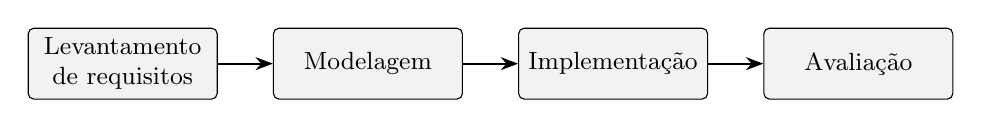
\begin{tikzpicture}[node distance=7mm, font=\small,
        etapa/.style={draw, rounded corners=2pt, minimum height=9mm, minimum width=24mm,
                      align=center, fill=black!5},
        seta/.style={-{Stealth[length=2.2mm]}, thick}]
      \node[etapa] (a) {Levantamento\\de requisitos};
      \node[etapa, right=of a] (b) {Modelagem};
      \node[etapa, right=of b] (c) {Implementação};
      \node[etapa, right=of c] (d) {Avaliação};
      \draw[seta] (a) -- (b);
      \draw[seta] (b) -- (c);
      \draw[seta] (c) -- (d);
    \end{tikzpicture}
  \end{ilustracao}
\end{figure}

\begin{dica}[Dica de uso da classe: figuras]
Na ilustração, o \emph{cabeçalho} (tipo, número e título) é centralizado, acima, e o
\emph{rodapé} (fonte, legenda e notas) fica abaixo, alinhado à margem esquerda da
própria ilustração, em espaço simples e tamanho 10 (manual UFV 4.9). O ambiente
\texttt{ilustracao}, do \texttt{abntex2-ufv}, mede o conteúdo e cuida disso. Use-o dentro
do \texttt{figure}, com os argumentos na ordem \emph{título} e \emph{rodapé}:
\texttt{\textbackslash begin\{ilustracao\}\allowbreak\{\textbackslash caption\{Título\}\allowbreak\textbackslash label\{rótulo\}\}\allowbreak\{\textbackslash fonte\{Fonte\}\allowbreak\textbackslash nota\{Nota\}\}},
com o \texttt{\textbackslash includegraphics} ou o diagrama dentro. As imagens ficam na
pasta \texttt{imagens/}, ao lado do arquivo principal: a classe já configura o
\texttt{\textbackslash graphicspath}, então basta
\texttt{\textbackslash includegraphics\{arquivo\}}, sem o nome da pasta. Para a fonte de autoria
própria, use \texttt{\textbackslash elaboracaopropria}. Com
\texttt{\textbackslash caption[título curto]\{título longo\}}, a lista de ilustrações
recebe o nome curto. Prefira \ac{pdf} ou \ac{svg} convertido (vetoriais) para diagramas e
\ac{png} com pelo menos 300 dpi para capturas de tela, e sempre cite a figura no texto,
com \texttt{\textbackslash autoref}. Diagramas simples podem ser desenhados no próprio
\LaTeX\ com TikZ, como a \autoref{fig:etapas}.
\end{dica}

A \autoref{fig:logo} mostra a inserção de uma imagem; quando a imagem não é de autoria
própria, indique a fonte com \texttt{\textbackslash fonte} e inclua a obra nas referências.

\begin{figure}[htbp]
  \begin{ilustracao}{\caption[Exemplo de figura]{Exemplo de inserção de figura no \LaTeX}\label{fig:logo}}{\fonte{Universidade Federal de Viçosa (adaptado)}\nota{A imagem é um exemplo e deve ser substituída.}}
    
\includegraphics[width=.7\linewidth]{Logo_Sistemas}
  \end{ilustracao}
\end{figure}

\section{Código-fonte}

Trechos de programa usam o ambiente \texttt{codigo}, que gera a ``Lista de códigos''
(\autoref{cod:exemplo}), como esta consulta \ac{sql} enviada a um \ac{sgbd} por meio de
uma \ac{api}. Programas extensos devem ir para apêndice ou repositório.

\begin{codigo}[htbp]
\begin{ilustracao}[\linewidth]{\caption{Exemplo de consulta SQL}\label{cod:exemplo}}{\elaboracaopropria}
\begin{lstlisting}[language=SQL, frame=tb]
SELECT nome, COUNT(*) AS total
FROM aluno
GROUP BY nome
ORDER BY total DESC;
\end{lstlisting}
\end{ilustracao}
\end{codigo}

\begin{dica}[Dica de uso da classe: código-fonte]
Escreva o código dentro de \texttt{lstlisting} (pacote \texttt{listings}) e informe a
linguagem em \texttt{[language=...]}. O ambiente \texttt{codigo}, definido pelo
\texttt{abntex2-ufv}, cria o rótulo ``Código N'' e a lista própria. Como a moldura do
\texttt{lstlisting} ocupa a largura da página, use
\texttt{\textbackslash begin\{ilustracao\}[\textbackslash linewidth]\{...\}\{...\}}: o argumento
opcional dá a largura mínima do título e do rodapé.
Para código com muitas linhas, \texttt{\textbackslash lstinputlisting\{arquivo.py\}}
lê o arquivo diretamente.
\end{dica}

\chapter{Resultados e Discussão}\label{sec:resultados}

\begin{dica}[Dica de metodologia científica: resultados e discussão]
Apresente primeiro os resultados, de forma objetiva e na ordem dos objetivos
específicos; depois discuta-os. Na discussão: interprete os números (o que significam?),
compare com os trabalhos do Referencial Teórico (confirmam ou contradizem?), relacione
com os objetivos e reconheça as limitações. Use tabelas, quadros e gráficos para os
dados e comente-os no texto \emph{sem repeti-los}: destaque o que importa. Toda
ilustração deve ser citada e explicada no texto. Resultados negativos ou inesperados
também são resultados e devem ser relatados e discutidos.
\end{dica}

\section{Tabelas}

Tabelas apresentam dados em que o \emph{número} é a informação central e seguem as
normas de apresentação tabular do \ac{ibge}. A \autoref{tab:exemplo} mostra o formato:
título acima, sem linhas verticais, fonte abaixo.

Nela, as colunas numéricas (tipo \texttt{S} do pacote \texttt{siunitx})
são alinhadas \emph{pela vírgula decimal}, mesmo quando os números têm quantidades
diferentes de dígitos e de casas decimais (``1234,5'' e ``62,8''; ``112,40'' e ``18,70''),
e os milhares são separados por ponto (``14.820''). A tabela ocupa toda a largura do
texto, e o título e o rodapé acompanham essa largura.

\begin{table}[htbp]
\begin{tabela}[\linewidth]{\caption{Desempenho das operações do sistema em cinco métricas}\label{tab:exemplo}}{\elaboracaopropria\nota{Média de 30 execuções. A coluna ``Variação'' compara com a versão anterior; valores negativos indicam melhoria.}}
  \begin{tabular*}{\linewidth}{@{\extracolsep{\fill}} l S[table-format=4.1] S[table-format=3.1] S[table-format=3.2] S[table-format=5.0] S[table-format=-2.1]}
    \toprule
    \textbf{Operação} & {\textbf{Tempo (ms)}} & {\textbf{Desvio (ms)}} & {\textbf{Memória (MB)}} & {\textbf{Vazão (req/s)}} & {\textbf{Variação (\%)}} \\
    \midrule
    Cadastro de usuário  &  184,3 &  12,6 &  41,25 &   520 &  -8,4 \\
    Autenticação         &   62,8 &   4,1 &  18,70 & 14820 & -12,0 \\
    Busca simples        &   95,5 &   7,9 &  33,05 &  9600 &  -3,2 \\
    Busca avançada       & 1234,5 &  85,2 & 112,40 &    78 &   5,7 \\
    Relatório mensal     & 2310,0 & 140,8 & 256,10 &    12 &  -0,6 \\
    Envio de arquivo     &  845,7 &  63,4 &  96,35 &   140 &   2,3 \\
    Exportação em CSV    &  530,2 &  38,9 &  64,80 &   260 & -21,5 \\
    Notificação por e-mail & 71,6 &   5,3 &  22,15 &  7800 &   0,0 \\
    Consulta de histórico &  318,9 & 24,7 &  52,45 &   460 &   9,8 \\
    \bottomrule
  \end{tabular*}
\end{tabela}
\end{table}

\begin{dica}[Dica de uso da classe: tabelas e quadros]
Se o conteúdo é \emph{numérico}, é \textbf{tabela}; se é \emph{textual}
(comparações, requisitos, definições, códigos), é \textbf{quadro}. As duas coisas têm
listas, numerações e formatos diferentes, por isso não classifique tudo como tabela. O
Apêndice~\ref{ap:tabelas} traz exemplos completos de tabelas e quadros bem formatados
e os principais ajustes (largura, alinhamento, notas, tabelas longas, células mescladas).
\end{dica}

\section{Gráficos}

Gráficos têm lista própria (``Lista de gráficos''). O \autoref{gra:exemplo} foi
desenhado no próprio \LaTeX\ com o pacote \texttt{pgfplots}, que funciona sobre o TikZ
(por isso o ambiente \texttt{axis} fica dentro de um \texttt{tikzpicture}), o que mantém
fontes e tamanhos coerentes com o texto.

\begin{grafico}[htbp]
  \begin{ilustracao}{\caption{Tempo médio de resposta por implementação}\label{gra:exemplo}}{\elaboracaopropria\nota{Média de 30 execuções.}}
    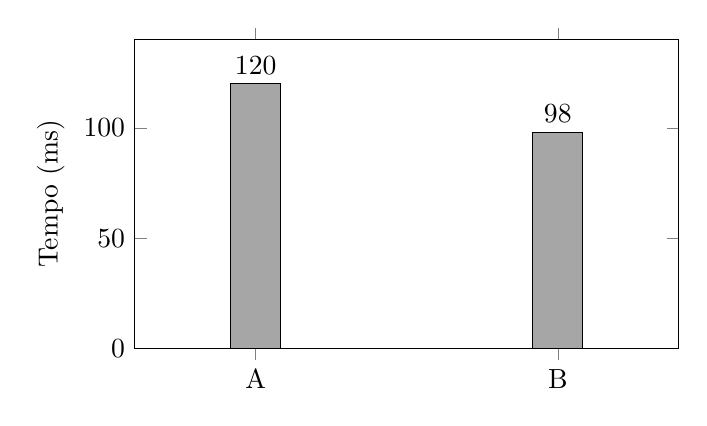
\begin{tikzpicture}
      \begin{axis}[ybar, width=0.7\linewidth, height=5.5cm, bar width=18pt,
          symbolic x coords={A, B}, xtick=data, ymin=0, ymax=140,
          ylabel={Tempo (ms)}, nodes near coords, enlarge x limits=0.4]
        \addplot[fill=black!35] coordinates {(A,120) (B,98)};
      \end{axis}
    \end{tikzpicture}
  \end{ilustracao}
\end{grafico}

\chapter{Conclusão}\label{sec:conclusao}

\begin{dica}[Dica de metodologia científica: o que escrever na Conclusão]
A conclusão \emph{responde} aos objetivos: retome o objetivo geral e, um a um, os
específicos, dizendo o que foi alcançado e apontando a evidência (seção, resultado,
artefato). Em seguida: (i) as \textbf{contribuições} do trabalho; (ii) as
\textbf{limitações} (o que não foi feito ou não pode ser generalizado); e (iii) os
\textbf{trabalhos futuros}, de forma concreta. Não introduza dados, figuras ou citações
novas, não repita a introdução nem termine com frases genéricas. O texto deve ser
compreensível para quem leu apenas a introdução e a conclusão.
\end{dica}

Apresente as conclusões correspondentes aos objetivos ou hipóteses, as limitações e
os trabalhos futuros.

% Use apenas no projeto (TCC I). Remova o \input correspondente na monografia final.
\chapter{Cronograma}\label{sec:cronograma}

\begin{dica}[Dica de metodologia científica: cronograma]
O cronograma mostra que o trabalho é viável: liste as atividades na ordem lógica
(revisão bibliográfica, levantamento de requisitos, modelagem, implementação, testes,
escrita, defesa), com duração realista e margem para imprevistos, e relacione-as aos
objetivos específicos. Em \ac{tcc} I (projeto), o cronograma é elemento esperado; na
monografia final, em geral, é suprimido. Como o cronograma não traz dados numéricos,
ele é um \textbf{quadro} (e não uma tabela); diagramas (Gantt e PERT/CPM) são
\textbf{figuras}.
\end{dica}

\begin{dica}[Dica de uso da classe: quatro formas de apresentar o cronograma]
Escolha \emph{uma} das formas abaixo. As duas primeiras são quadros (\texttt{quadro} com
\texttt{ilustracao}): marcas nos meses e células sombreadas (pacote \texttt{colortbl}), que
imprime bem em preto e branco. As duas últimas são figuras desenhadas com TikZ: o diagrama
de Gantt (desenhado em TikZ) mostra as atividades como barras ao longo do tempo, e
o diagrama PERT/CPM mostra as \emph{dependências} entre as atividades, as folgas e o caminho
crítico, sendo o mais adequado quando a ordem de execução importa. Em todos os exemplos o
objeto ocupa a largura do texto sem alterar o tamanho da letra: o primeiro e o segundo usam
\texttt{tabularx} com uma coluna \texttt{X} elástica; o terceiro calcula a unidade horizontal
a partir de \texttt{\textbackslash linewidth}; o quarto distribui os nós na largura. Em
qualquer caso a fonte é obrigatória e a legenda explica o símbolo usado.
\end{dica}

\section{Opção A: quadro com marcas}

O cronograma das atividades é apresentado no \autoref{qua:cronograma}.

\begin{quadro}[htbp]
\begin{ilustracao}[\linewidth]{\caption{Cronograma do projeto em meses}\label{qua:cronograma}}{\elaboracaopropria\legenda{O símbolo $\bullet$ indica o mês em que a atividade é executada.}}
  \small
  \begin{tabularx}{\linewidth}{|l|*{12}{>{\centering\arraybackslash}X|}}
    \hline
    \textbf{Atividade} & \textbf{1} & \textbf{2} & \textbf{3} & \textbf{4} & \textbf{5} & \textbf{6} & \textbf{7} & \textbf{8} & \textbf{9} & \textbf{10} & \textbf{11} & \textbf{12} \\
    \hline
    Revisão bibliográfica & $\bullet$ & $\bullet$ & & & & & & & & & & \\
    \hline
    Métodos & & & $\bullet$ & $\bullet$ & & & & & & & & \\
    \hline
    Testes & & & & $\bullet$ & $\bullet$ & $\bullet$ & & & & & & \\
    \hline
    Resultados & & & & & & & $\bullet$ & $\bullet$ & & & & \\
    \hline
    Conclusão & & & & & & & $\bullet$ & $\bullet$ & $\bullet$ & & & \\
    \hline
    Banca & & & & & & & & & & $\bullet$ & $\bullet$ & $\bullet$ \\
    \hline
  \end{tabularx}
\end{ilustracao}
\end{quadro}

\section{Opção B: quadro com células sombreadas}

O \autoref{qua:cronograma-cor} traz o mesmo cronograma com as células do período
sombreadas, com o cabeçalho ``Mês'' agrupando as doze colunas e linhas mais altas para
melhorar a leitura.

\newcommand{\mes}{\cellcolor{black!35}}

\begin{quadro}[htbp]
\begin{ilustracao}[\linewidth]{\caption{Cronograma do projeto com células sombreadas}\label{qua:cronograma-cor}}{\elaboracaopropria\legenda{As células sombreadas indicam os meses de execução de cada atividade.}}
  \small
  \renewcommand{\arraystretch}{1.5}
  \begin{tabularx}{\linewidth}{|l|*{12}{>{\centering\arraybackslash}X|}}
    \hline
    \multirow{2}{*}{\textbf{Atividade}} & \multicolumn{12}{c|}{\textbf{Mês}} \\
    \cline{2-13}
     & 1 & 2 & 3 & 4 & 5 & 6 & 7 & 8 & 9 & 10 & 11 & 12 \\
    \hline
    Revisão bibliográfica & \mes & \mes & & & & & & & & & & \\
    \hline
    Métodos & & & \mes & \mes & & & & & & & & \\
    \hline
    Testes & & & & \mes & \mes & \mes & & & & & & \\
    \hline
    Resultados & & & & & & & \mes & \mes & & & & \\
    \hline
    Conclusão & & & & & & & \mes & \mes & \mes & & & \\
    \hline
    Banca & & & & & & & & & & \mes & \mes & \mes \\
    \hline
  \end{tabularx}
\end{ilustracao}
\end{quadro}

\section{Opção C: diagrama de Gantt}

A \autoref{fig:gantt} apresenta o cronograma como um diagrama de Gantt, que mostra as
atividades como barras ao longo do tempo e deixa evidentes as sobreposições. Ele é
desenhado diretamente em TikZ, em uma grade única: os nomes das atividades ficam
\emph{dentro} da moldura, em uma primeira coluna, e o diagrama ocupa toda a largura do
texto (a largura de cada mês é calculada a partir de \texttt{\textbackslash linewidth}).
Para mudar as atividades, edite a lista do \texttt{\textbackslash foreach} no formato
\texttt{nome/mês inicial/mês final} e ajuste \texttt{\textbackslash ufvnativ} (número de
atividades).

\begin{figure}[htbp]
\begin{ilustracao}[\linewidth]{\caption{Diagrama de Gantt do cronograma do projeto}\label{fig:gantt}}{\elaboracaopropria\legenda{Cada barra indica a duração da atividade, em meses.}}
  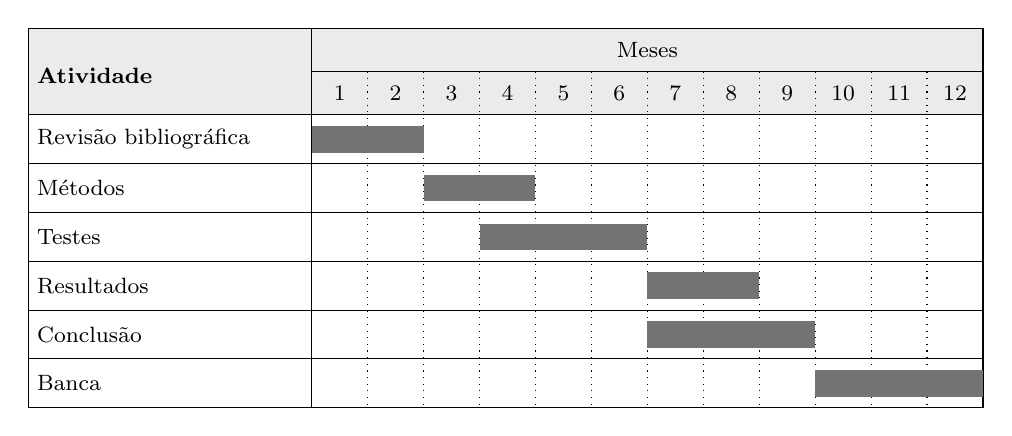
\begin{tikzpicture}[font=\footnotesize, line width=0.4pt]
    \def\ufvnativ{6}                                      % número de atividades
    \pgfmathsetlengthmacro{\ufvlc}{3.6cm}                 % largura da coluna de atividades
    \pgfmathsetlengthmacro{\ufvxu}{(\linewidth-\ufvlc)/12} % largura de cada mês
    \pgfmathsetlengthmacro{\ufvhh}{1.1cm}                 % altura do cabeçalho (2 linhas)
    \pgfmathsetlengthmacro{\ufvrh}{0.62cm}                % altura de cada atividade
    \pgfmathsetlengthmacro{\ufvht}{\ufvhh+\ufvnativ*\ufvrh} % altura total
    % cabeçalho sombreado, moldura e linhas
    \fill[black!8] (0,0) rectangle (\linewidth,-\ufvhh);
    \draw (0,0) rectangle (\linewidth,-\ufvht);
    \draw (0,-\ufvhh) -- (\linewidth,-\ufvhh);
    \draw (\ufvlc,0) -- (\ufvlc,-\ufvht);
    \draw (\ufvlc,-0.55cm) -- (\linewidth,-0.55cm);
    \node[anchor=west, inner xsep=3pt, font=\footnotesize\bfseries] at (0,-0.55*\ufvhh) {Atividade};
    \node at ({\ufvlc+6*\ufvxu},-0.275cm) {Meses};
    \foreach \m in {1,...,12} {
      \node at ({\ufvlc+(\m-0.5)*\ufvxu},-0.825cm) {\m};
      \draw[dotted] ({\ufvlc+\m*\ufvxu},-0.55cm) -- ({\ufvlc+\m*\ufvxu},-\ufvht);
    }
    % atividades: nome/mês inicial/mês final
    \foreach \nome/\ini/\fim [count=\k] in {Revisão bibliográfica/1/2, Métodos/3/4,
        Testes/4/6, Resultados/7/8, Conclusão/7/9, Banca/10/12} {
      \pgfmathsetlengthmacro{\yt}{-\ufvhh-(\k-1)*\ufvrh}
      \draw (0,\yt) -- (\linewidth,\yt);
      \node[anchor=west, inner xsep=3pt] at (0,\yt-0.5*\ufvrh) {\nome};
      \fill[black!55] ({\ufvlc+(\ini-1)*\ufvxu},\yt-0.14cm) rectangle ({\ufvlc+\fim*\ufvxu},\yt-\ufvrh+0.14cm);
    }
  \end{tikzpicture}
\end{ilustracao}
\end{figure}
  % apenas no projeto (TCC I)

% ----------------------------------------------------------
% ELEMENTOS PÓS-TEXTUAIS
% ----------------------------------------------------------
\postextual

% Referências (as entradas de exemplo, com keywords = {guia}, não são impressas)
\printbibliography[notkeyword=guia]

% Glossário (opcional): relação de termos técnicos com suas definições
\begin{glossario}
\termo{Caso de uso}{descrição de uma interação entre um ator e o sistema para atingir
  um objetivo, usada no levantamento e na modelagem de requisitos.}
\termo{Requisito funcional}{funcionalidade ou comportamento que o sistema deve oferecer.}
\termo{Requisito não funcional}{restrição ou qualidade exigida do sistema, como
  desempenho, segurança ou usabilidade.}
\end{glossario}

% Apêndices (texto elaborado pelo autor) e anexos (documentos de terceiros).
\begin{apendicesenv}
\partapendices
% Apêndice do exemplo: guia de referências e citações. Apague-o no seu trabalho
% (e remova example-entradas.bib do preâmbulo).

% Exibe uma entrada de exemplo (trecho do arquivo example-entradas.bib entre as
% marcas @comment{BEGIN:#1} e @comment{END:#1}) e o resultado impresso (\fullcite)
% da chave #2.
% Uso: \refex{marcador}{chave}{descrição}
\newcommand{\refex}[3]{%
  \par\medskip\noindent\textbf{#3}\par\nopagebreak\smallskip
  \lstinputlisting[style=exemplo, language=BibTeX, linerange={BEGIN:#1-END:#1},
                   rangeprefix=@comment\{, rangesuffix=\}, includerangemarker=false]%
                  {example/example-entradas.bib}%
  \par\nopagebreak\smallskip\noindent\textit{Resultado na lista de referências:}\par\nopagebreak
  \begin{SingleSpacing}\noindent\hspace{1cm}\begin{minipage}{0.9\textwidth}%
    \raggedright\fullcite{#2}.\end{minipage}\end{SingleSpacing}\par\medskip}

\chapter{Guia de referências e citações}\label{ap:referencias}

Este apêndice mostra como escrever as entradas do arquivo \texttt{referencias.bib}
para os tipos de documento mais usados em trabalhos de computação e o resultado que
elas produzem na lista de referências, conforme o Manual de Normalização de Trabalhos
Acadêmicos da \ac{ufv} \cite{manualUFV}, a NBR 6023/2025 (referências) e a NBR 10520/2023
(citações). Os exemplos vêm do arquivo \texttt{example-entradas.bib}: parte deles
reproduz exemplos do manual; os demais têm dados ilustrativos.

\section{Regras gerais}

\begin{itemize}
  \item As referências ficam em \textbf{uma única lista}, em ordem alfabética, em
        espaço simples, alinhadas à margem esquerda e separadas por uma linha em branco.
        O estilo \texttt{abnt} do biblatex faz tudo isso automaticamente.
  \item Entram na lista \textbf{somente as obras citadas} no texto. (Obras apenas
        lidas, sem citação, formariam uma \emph{bibliografia}, outro elemento.)
  \item O \textbf{destaque tipográfico do título} (aqui, negrito) deve ser o mesmo em
        todas as referências; ele não se aplica às obras sem autoria, cuja entrada é o
        título, já destacado pelas maiúsculas na primeira palavra.
  \item O autor é indicado pelo último sobrenome em maiúsculas, seguido do prenome
        (por extenso ou abreviado, \textbf{de forma uniforme}). Até três autores,
        todos; com quatro ou mais, indicam-se todos ou só o primeiro seguido de
        \emph{et al.} (este modelo usa \emph{et al.}).
  \item Documentos \emph{online} levam, ao final, \textbf{Disponível em:} (endereço) e
        \textbf{Acesso em:} (data de acesso).
  \item Quando um elemento não aparece na obra, mas pode ser identificado, vai entre
        colchetes: \texttt{[Cupertino]}. Se não puder ser identificado, usam-se
        \texttt{[S. l.]} (local) e \texttt{[s. n.]} (editora).
\end{itemize}

\section{Campos mais usados}

O \autoref{qua:campos} resume os campos do \texttt{.bib} usados nos exemplos. Escreva
os nomes como \emph{Sobrenome, Prenome} e separe os autores com \texttt{and}. Para
entidades (autor institucional), use chaves duplas, que impedem a inversão do nome:
\texttt{author = \{\{Universidade Federal de Viçosa\}\}}. O campo \texttt{doi} recebe
apenas o número do \ac{doi}, sem o prefixo de endereço.

\begin{quadro}[htbp]
\begin{ilustracao}{\caption{Campos do biblatex mais usados nas entradas}\label{qua:campos}}{\fonte{Elaborado pelo próprio autor}}
  \renewcommand{\arraystretch}{1.2}
  \small
  \begin{tabularx}{\textwidth}{|>{\ttfamily\raggedright\arraybackslash}p{3.2cm}|X|}
    \hline
    \textnormal{\textbf{Campo}} & \textbf{Uso} \\
    \hline
    author, editor & Autores (\texttt{Sobrenome, Prenome and ...}) e organizadores/editores \\
    \hline
    title, subtitle & Título e subtítulo; o subtítulo é impresso após dois-pontos \\
    \hline
    edition & Número da edição (\texttt{2} gera ``2. ed.''); texto livre vira o próprio texto \\
    \hline
    location, publisher & Local (cidade) e editora, sem natureza jurídica (``Editora Atlas'' $\to$ ``Atlas'') \\
    \hline
    year, date & Ano ou data completa (\texttt{2003-11/2003-12} gera ``nov./dez. 2003'') \\
    \hline
    pages, pagetotal & Páginas inicial e final (\texttt{15--24}) e número total de páginas \\
    \hline
    journaltitle, volume, number & Periódico, volume e fascículo (artigos) \\
    \hline
    doi, url, urldate & DOI, endereço eletrônico e data de acesso (\texttt{AAAA-MM-DD}) \\
    \hline
    type, institution, eventdate & Trabalhos acadêmicos: tipo (grau e curso), instituição e data da defesa \\
    \hline
    eventtitle, venue & Eventos: nome do evento e cidade de realização \\
    \hline
    shorttitle & Título curto, usado na citação de obras sem autoria \\
    \hline
    keywords & Palavras-chave internas (nos exemplos, \texttt{guia}) \\
    \hline
  \end{tabularx}
\end{ilustracao}
\end{quadro}

\section{Convenções do estilo \texttt{abnt}}

O pacote \texttt{biblatex-abnt} segue a NBR 6023, mas algumas formas só saem certas
com estas convenções (já adotadas nos exemplos abaixo):
\begin{alineas}
  \item \textbf{trabalhos acadêmicos}: use \texttt{@thesis} e informe a data da defesa
        em \texttt{eventdate}, que é impressa ao final (``\ldots\ Universidade, Local, ano'');
  \item \textbf{documentos online com local e editora}: use \texttt{@book} (ou
        \texttt{@misc}) com \texttt{url} e \texttt{urldate}; \texttt{@online} não imprime
        local nem editora;
  \item \textbf{obras sem autoria}: omita \texttt{author}; se o título começar por
        artigo ou monossílabo, preencha \texttt{shorttitle} (ver a Seção~\ref{sec:semautoria});
  \item \textbf{local ou editora desconhecidos}: escreva \texttt{[S. l.]} ou \texttt{[s. n.]}
        no próprio campo;
  \item \textbf{autor institucional}: use chaves duplas,
        \texttt{author = \{\{Universidade Federal de Viçosa\}\}}. Com chaves simples, o
        biblatex trata ``Viçosa'' como sobrenome e imprime \emph{VIÇOSA, U. F. de.} na lista e
        ``(Viçosa, 1999)'' na citação, o que está errado.
\end{alineas}

\section{Livros}

\refex{livro}{ex-livro}{Livro com um autor}
\refex{livro_3}{ex-livro-3}{Livro com três autores (todos são indicados)}
\refex{livro_4}{ex-livro-4}{Livro com quatro ou mais autores (primeiro autor e \emph{et al.})}
\refex{livro_org}{ex-livro-org}{Livro com organizador}
\refex{livro_trad}{ex-livro-trad}{Livro com tradutor, número de páginas e \ac{isbn} (elementos complementares)}

\section{Partes de livros}

\refex{capitulo}{ex-capitulo}{Capítulo de livro do mesmo autor}
\refex{capitulo_org}{ex-capitulo-org}{Capítulo de livro organizado por outros autores}

\section{Trabalhos acadêmicos (TCC, dissertação e tese)}

\refex{tcc}{ex-tcc}{Trabalho de conclusão de curso}
\refex{dissertacao}{ex-dissertacao}{Dissertação}
\refex{tese}{ex-tese}{Tese}

\begingroup\sloppy
Para um \ac{tcc} do curso de Sistemas de Informação da \ac{ufv}, o campo \texttt{type} fica
``\texttt{Trabalho de Conclusão de Curso (Bacharelado em Sistemas de Informação)}'' e
\texttt{institution} fica
``\texttt{Instituto de Ciências Exatas e Tecnológicas, Universidade Federal de Viçosa}'' (ou o nome da unidade do seu \emph{campus}).\par\endgroup

\section{Artigos de periódicos}

\refex{artigo}{ex-artigo}{Artigo de periódico, versão impressa}
\refex{artigo_online}{ex-artigo-online}{Artigo de periódico \emph{online}, com DOI, endereço e data de acesso}

\section{Trabalhos apresentados em eventos}

\refex{evento}{ex-evento}{Trabalho em evento (\texttt{@inproceedings}); \texttt{number} é o número da edição do evento}

\section{Normas, legislação e documentos institucionais}

\refex{norma}{ex-norma}{Norma técnica}
\refex{legislacao}{ex-legislacao}{Legislação disponível \emph{online}: o autor é a jurisdição (Brasil, estado ou município); o nome e a data da lei ficam fora do negrito (\texttt{\textbackslash textmd\{...\}}) e só a ementa é destacada}

Este modelo cobre a legislação (seção 5.12.16.1 e 5.12.16.2 do manual). A jurisprudência
(acórdãos, súmulas) e os atos administrativos normativos (portarias, resoluções) têm
elementos próprios, como tribunal, número do processo e relator, que o estilo \texttt{abnt}
não cobre por completo; para eles, siga o manual (seções 5.12.16.3 a 5.12.16.6). Pode ser necessário usar
\texttt{@misc} e montar parte do texto nos campos \texttt{title} e \texttt{note}; confira
sempre o resultado impresso contra os exemplos do manual.
\refex{entidade}{ex-entidade}{Autor institucional (a entidade é o autor)}
\refex{relatorio}{ex-relatorio}{Relatório de organização (publicação em meio eletrônico, com data completa)}

\section{Documentos \emph{online}, repositórios e programas}

\refex{site}{ex-site}{Página \emph{web} (use \texttt{[S. l.]} se o local não é identificado)}
\refex{repositorio}{ex-repositorio}{Repositório de código}
\refex{software}{ex-software}{Programa de computador (a versão fica no campo \texttt{edition})}

\section{Obras sem autoria}\label{sec:semautoria}

\refex{sem_autor}{ex-sem-autor}{Título como entrada (primeira palavra em maiúsculas na lista)}
\refex{sem_autor_artigo}{ex-sem-autor-artigo}{Título iniciado por artigo: escreva em maiúsculas o artigo e a palavra seguinte, e use \texttt{shorttitle}}

\section{Citações no texto}\label{sec:citacoes}

O sistema de chamada adotado é o \textbf{autor-data} (NBR 10520:2023). O sistema
numérico não pode ser usado quando há notas. O \autoref{qua:citacoes} mostra os
comandos e o resultado para os casos mais comuns.

\begin{quadro}[htbp]
\begin{ilustracao}{\caption{Comandos de citação e resultado}\label{qua:citacoes}}{\fonte{Elaborado pelo próprio autor}}
  \renewcommand{\arraystretch}{1.2}
  \small
  \begin{tabularx}{\textwidth}{|>{\ttfamily\raggedright\arraybackslash}p{6.4cm}|X|}
    \hline
    \textnormal{\textbf{Comando}} & \textbf{Resultado} \\
    \hline
    \textbackslash cite\{ex-livro\} & \cite{ex-livro} (um autor) \\
    \hline
    \textbackslash cite[p.~35]\{ex-livro\} & \cite[p.~35]{ex-livro} (com página) \\
    \hline
    \textbackslash cite\{ex-livro,ex-artigo\} & \cite{ex-livro,ex-artigo} (várias obras, em ordem alfabética) \\
    \hline
    \textbackslash cite\{ex-livro-3\} & \cite{ex-livro-3} (três autores) \\
    \hline
    \textbackslash cite\{ex-livro-4\} & \cite{ex-livro-4} (quatro ou mais autores) \\
    \hline
    \textbackslash textcite\{ex-livro\} & \textcite{ex-livro} (no fluxo da frase) \\
    \hline
    \textbackslash textcite[p.~35]\{ex-livro-3\} & \textcite[p.~35]{ex-livro-3} \\
    \hline
    \textbackslash cite\{ex-entidade\} & \cite{ex-entidade} (autor institucional) \\
    \hline
    \textbackslash cite\{ex-norma\} & \cite{ex-norma} \\
    \hline
    \textbackslash cite\{ex-sem-autor\} & \cite{ex-sem-autor} (sem autoria) \\
    \hline
    \textbackslash cite\{ex-sem-autor-artigo\} & \cite{ex-sem-autor-artigo} (sem autoria, com \texttt{shorttitle}) \\
    \hline
    \textbackslash cite\{ex-reeside-a,\allowbreak ex-reeside-b\} & \cite{ex-reeside-a,ex-reeside-b} (mesmo autor e ano: letras a, b) \\
    \hline
    \textbackslash textapud\{ex-livro\}\{ex-livro-3\} & \textapud{ex-livro}{ex-livro-3} (citação de citação; só a obra consultada entra na lista) \\
    \hline
  \end{tabularx}
\end{ilustracao}
\end{quadro}

Outras regras da NBR 10520:2023 que o manual da \ac{ufv} destaca:
\begin{itemize}
  \item \textbf{supressões} no trecho citado são indicadas por \texttt{[...]};
        interpolações e comentários, por \texttt{[~~]}; ênfase por sublinhado, negrito ou
        itálico, seguida de ``\emph{grifo nosso}'' ou ``\emph{grifo próprio}'' na chamada;
  \item \textbf{tradução} própria de trecho citado: acrescente \emph{tradução nossa} na chamada;
  \item citações diretas de documento \textbf{sem paginação} indicam a localização do
        trecho (\texttt{local.}, capítulo, artigo etc.);
  \item o \textbf{ponto final} encerra a frase, não a citação.
\end{itemize}

\section{Dicas de uso do arquivo \texttt{.bib}}

\begin{itemize}
  \item \textbf{Chaves}: use chaves curtas e padronizadas (\texttt{silva2024}, sem acentos
        nem espaços). Cada chave é única.
  \item \textbf{Codificação}: o arquivo deve estar em UTF-8; acentos são digitados normalmente.
  \item \textbf{Maiúsculas}: o estilo decide a caixa dos títulos; para preservar uma sigla
        ou nome próprio, use chaves: \texttt{title = \{Uso de \{Python\} em \{SGBD\}\}}.
  \item \textbf{Gerenciadores}: Zotero e JabRef exportam \texttt{.bib}; confira os campos
        exportados com este guia, pois nem sempre seguem as convenções acima.
  \item \textbf{Compilação}: após incluir ou alterar citações, rode
        \texttt{pdflatex}, \texttt{biber}, \texttt{pdflatex}, \texttt{pdflatex} (ou
        simplesmente \texttt{latexmk -pdf}). ``Citation \ldots\ undefined'' ou ``(?)''
        indica que o \texttt{biber} ainda não foi executado ou que a chave está errada.
\end{itemize}

% Apêndice do modelo: guia de tabelas e quadros. Apague-o no seu trabalho
% (e a pasta apendices/exemplos).

% Mostra o código de example/snippets/#1.tex e o resultado (o mesmo arquivo, incluído).
% Para que o resultado fique junto do código (e não flutue para outra página), aqui os
% ambientes figure, table, quadro, grafico e codigo são redefinidos localmente como blocos
% fixos (não flutuantes); \caption, \label e \autoref continuam funcionando.
% Em um trabalho real use os floats normais ([htbp]), como mostram os códigos exibidos.
\makeatletter
\newcommand{\ufv@semfloat}[1]{%
  \renewenvironment{#1}[1][]{\par\medskip\begin{minipage}{\linewidth}\def\@captype{#1}}%
    {\end{minipage}\par\medskip}}
\newcommand{\ufv@modofixo}{\ufv@semfloat{table}\ufv@semfloat{figure}\ufv@semfloat{quadro}%
  \ufv@semfloat{grafico}\ufv@semfloat{codigo}}
\newcommand{\codexemplo}[1]{%
  \par\medskip\noindent\textit{Código:}\par\nopagebreak\smallskip
  \lstinputlisting[style=exemplo, language={[LaTeX]TeX}]{example/snippets/#1.tex}%
  \par\medskip
  \noindent\begin{minipage}{\linewidth}\textit{Resultado:}\par\nopagebreak\smallskip
  \begingroup\ufv@modofixo\input{example/snippets/#1}\endgroup
  \end{minipage}\par}
% variante para tabelas longas (longtable precisa quebrar página): mostra só as primeiras
% linhas do código (#2 = última linha exibida) e não coloca o resultado em bloco
\newcommand{\codexemplolongo}[2]{%
  \par\medskip\noindent\textit{Código (primeiras linhas; as demais seguem o mesmo padrão):}\par\nopagebreak\smallskip
  \lstinputlisting[style=exemplo, language={[LaTeX]TeX}, lastline=#2]{example/snippets/#1.tex}%
  \par\medskip\noindent\textit{Resultado:}\par\nopagebreak\smallskip
  \input{example/snippets/#1}}
\makeatother

\chapter{Guia de tabelas e quadros}\label{ap:tabelas}

\emph{Observação}: nos exemplos deste apêndice, o código aparece primeiro e o resultado
logo abaixo, no mesmo lugar. Para isso, aqui os ambientes \texttt{table}, \texttt{figure},
\texttt{quadro}, \texttt{grafico} e \texttt{codigo} são exibidos como blocos fixos (sem
flutuar). Em um trabalho real, use-os normalmente, com \texttt{[htbp]}: o \LaTeX\ posiciona
o objeto perto do ponto em que ele é citado, e a referência no texto, feita com
\texttt{\textbackslash autoref\{rótulo\}}, continua correta mesmo que o objeto vá para outra
página, pois não depende da posição.

\section{Tabela ou quadro?}

Qualquer conteúdo organizado em linhas e colunas \emph{parece} uma tabela, mas as normas
distinguem os dois (NBR 14724; normas de apresentação tabular do \ac{ibge}). Classificar
tudo como tabela é um erro formal comum: as listas ficam erradas (itens textuais na
``Lista de tabelas'', por exemplo) e a apresentação foge do padrão. Isso não impede a
compilação nem a leitura, mas é o tipo de ajuste que a biblioteca ou a banca pode
exigir antes da versão final. Use o \autoref{qua:tabquadro} para decidir.

\begin{quadro}[htbp]
\begin{ilustracao}{\caption{Diferenças entre tabela e quadro}\label{qua:tabquadro}}{\fonte{Elaborado pelo próprio autor com base no manual da UFV}}
  \renewcommand{\arraystretch}{1.25}
  \small
  \begin{tabularx}{\textwidth}{|>{\raggedright\arraybackslash}p{2.8cm}|X|X|}
    \hline
    & \textbf{Tabela} & \textbf{Quadro} \\
    \hline
    Conteúdo & Dados numéricos; o número é a informação central (medidas, contagens, percentuais) & Informação textual ou mista: definições, requisitos, comparações, cronogramas, tecnologias \\
    \hline
    Bordas & Abertas nos lados: sem linhas verticais; linhas horizontais no topo, sob o cabeçalho e na base & Fechadas: linhas em todos os lados e entre as linhas e colunas \\
    \hline
    Ambientes & \texttt{table} com \texttt{tabela} (título à esquerda; equivale ao \texttt{\textbackslash IBGEtab}) & \texttt{quadro} com \texttt{ilustracao} (título centralizado) \\
    \hline
    Numeração e lista & ``Tabela N''; Lista de tabelas & ``Quadro N''; Lista de quadros \\
    \hline
    Rodapé & Abaixo, à esquerda: \texttt{\textbackslash fonte}, \texttt{\textbackslash legenda} e \texttt{\textbackslash nota} & O mesmo \\
    \hline
  \end{tabularx}
\end{ilustracao}
\end{quadro}

Regra prática: se você pode somar, comparar ou calcular com o conteúdo das células,
é tabela; se as células contêm frases, é quadro. Toda tabela e todo quadro devem ser
citados no texto (\texttt{\textbackslash autoref\{rótulo\}}) e ficar o mais perto possível
da citação.

\section{Título, fonte, legenda e nota}

Toda ilustração e toda tabela têm quatro elementos, nesta ordem (NBR 14724; manual UFV 4.9):
\begin{description}
  \item[Título] identifica o objeto, vem \emph{acima}, com a palavra designativa, o número,
        um travessão e o texto (``Figura 3 -- Arquitetura do sistema''); é o
        \texttt{\textbackslash caption}.
  \item[Fonte] indica de onde vem a informação e é \emph{obrigatória}, mesmo para obra do
        próprio autor (``Elaborado pelo próprio autor''); é o \texttt{\textbackslash fonte\{...\}}
        ou o atalho \texttt{\textbackslash elaboracaopropria}.
  \item[Legenda] explica símbolos, siglas, cores ou partes da ilustração (por exemplo,
        ``As células sombreadas indicam o período de execução''); é o \texttt{\textbackslash legenda\{...\}}
        e só é usada quando há algo a explicar.
  \item[Nota] traz observações e informações complementares (data da coleta, ressalvas,
        método); é o \texttt{\textbackslash nota\{...\}}.
\end{description}
Fonte, legenda e nota formam o \emph{rodapé}: ficam abaixo, em linhas seguidas, em espaço
simples, tamanho 10 e alinhadas à esquerda do objeto. A diferença para a tabela é só
o alinhamento do título: centralizado nas ilustrações e à esquerda nas tabelas (padrão do
\ac{ibge}).

\section{Os ambientes \texttt{ilustracao} e \texttt{tabela}}

Os dois ambientes têm a mesma sintaxe, parecida com a do \texttt{\textbackslash IBGEtab} do abn\TeX2:
título, conteúdo e rodapé, nessa ordem. Eles medem o conteúdo e montam título e rodapé na
largura dele:
\begin{lstlisting}[style=exemplo, language={[LaTeX]TeX}]
\begin{figure}[htbp]   % ou quadro, grafico, codigo
\begin{ilustracao}{\caption{Título}\label{fig:x}}{\fonte{...}\legenda{...}\nota{...}}
  \includegraphics[width=.8\linewidth]{figura}     % ou tikzpicture, tabularx, lstlisting
\end{ilustracao}
\end{figure}

\begin{table}[htbp]
\begin{tabela}{\caption{Título}\label{tab:x}}{\elaboracaopropria\nota{...}}
  \begin{tabular}{...} ... \end{tabular}
\end{tabela}
\end{table}
\end{lstlisting}
O \texttt{tabela} também reduz o conteúdo ao tamanho 10, como o \texttt{\textbackslash IBGEtab}
(para outro tamanho, redefina \texttt{\textbackslash IBGEtabfontsize}). O \texttt{\textbackslash IBGEtab}
do abn\TeX2 continua funcionando, mas não tem o espaçamento simples entre fonte e nota
nem aceita \texttt{\textbackslash legenda}.

\section{Tabela bem formatada}

Uma tabela no padrão \ac{ibge} usa o ambiente \texttt{tabela} dentro do \texttt{table}:
o título e o rodapé (fonte, legenda e notas) assumem a largura da tabela. As linhas
horizontais vêm do pacote \texttt{booktabs}
(\texttt{\textbackslash toprule}, \texttt{\textbackslash midrule},
\texttt{\textbackslash bottomrule}) e o alinhamento decimal da coluna \texttt{S} do
\texttt{siunitx}, configurada neste modelo para a vírgula decimal e o ponto
como separador de milhar. Entre as chaves \texttt{\{...\}}, os cabeçalhos das colunas
\texttt{S} protegem o texto da formatação numérica.

\codexemplo{tabela-simples}

Os principais ajustes:
\begin{itemize}
  \item \textbf{Alinhamento}: \sloppy texto à esquerda (\texttt{l}), números pela vírgula decimal
        (\texttt{S\allowbreak[table-format=3.1]}, em que o formato indica o máximo de dígitos antes e
        depois da vírgula), colunas centralizadas (\texttt{c}) só para códigos e marcas.
  \item \textbf{Unidades}: coloque a unidade no cabeçalho (``Tempo (ms)''), não em cada célula.
  \item \textbf{Largura}: se a tabela passa das margens, reduza a fonte com
        \texttt{\textbackslash small} ou \texttt{\textbackslash footnotesize} antes do
        \texttt{tabular} (o tamanho deve ser uniforme em todas as tabelas),
        diminua o espaço entre colunas com \texttt{\textbackslash setlength\{\textbackslash tabcolsep\}\{3pt\}}
        ou use \texttt{tabularx} com colunas \texttt{X}, que se ajustam à largura do texto.
        \texttt{\textbackslash resizebox\{\textbackslash textwidth\}\{!\}\{...\}} resolve, mas
        encolhe a letra de modo irregular: deixe como último recurso.
  \item \textbf{Altura das linhas}: \texttt{\textbackslash renewcommand\{\textbackslash arraystretch\}\{1.2\}}
        dá mais respiro às linhas (use dentro do ambiente, para não afetar o documento todo).
  \item \textbf{Células mescladas}: \texttt{\textbackslash multicolumn\allowbreak\{n\}\allowbreak\{c\}\allowbreak\{texto\}}
        (colunas) e \texttt{\textbackslash multirow\allowbreak\{n\}\allowbreak\{*\}\allowbreak\{texto\}} (linhas, pacote
        \texttt{multirow}); \texttt{\textbackslash cmidrule(lr)\{a-b\}} traça filetes parciais.
  \item \textbf{Sinais convencionais} (\ac{ibge}): hífen (--) para zero absoluto; três pontos
        (\ldots) para dado não disponível; \texttt{x} para dado omitido (consulte
        \cite{ibge1993} para a lista completa). Não deixe células vazias sem explicação.
  \item \textbf{Notas}: \texttt{\textbackslash nota\{...\}} explica a tabela como um todo;
        para notas de células específicas, use letras sobrescritas
        (\texttt{\textbackslash textsuperscript\{a\}}) e explique-as no rodapé.
  \item \textbf{Posição}: \texttt{[htbp]} deixa o \LaTeX\ escolher; não force posições
        (\texttt{[H]}), pois isso gera grandes espaços em branco.
\end{itemize}

\subsection{Células mescladas e cabeçalhos agrupados}

No exemplo a seguir comparam-se discos rígidos (\ac{hdd}) e unidades de estado sólido
(\ac{ssd}), com o cabeçalho ``Tempo (ms)'' agrupando as três colunas de medidas.

\codexemplo{tabela-mesclada}

\subsection{Tabela longa (mais de uma página)}

O ambiente \texttt{longtable} repete o cabeçalho em cada página e permite indicar a
continuação, como pedem as normas de apresentação tabular (``Continua'', ``Continuação''
e ``Conclusão'', conforme a posição). Use-o apenas quando a tabela realmente não couber
em uma página; tabelas longas e de consulta costumam ficar melhor em apêndice.

O \texttt{longtable} não é um float e não cabe dentro dos ambientes \texttt{table} e
\texttt{tabela}, por isso o título e o rodapé são tratados à parte:
\begin{itemize}
  \item o \textbf{título} é o \texttt{\textbackslash caption} da primeira linha da tabela. Para
        que fique à esquerda e use a largura do texto, coloque o \texttt{longtable} dentro de
        um grupo com
        \texttt{\textbackslash captionstyle\allowbreak[\textbackslash raggedright]\allowbreak\{\textbackslash raggedright\}} e
        \texttt{\textbackslash setlength\allowbreak\{\textbackslash LTcapwidth\}\allowbreak\{\textbackslash linewidth\}} (sem isso o
        título é limitado a 4 polegadas);
  \item para que o \textbf{rodapé} (\texttt{\textbackslash fonte}, \texttt{\textbackslash legenda} e
        \texttt{\textbackslash nota}) fique alinhado com a tabela, faça a tabela ocupar a largura do
        texto: \texttt{\textbackslash setlength\{\textbackslash LTleft\}\{0pt\}},
        \texttt{\textbackslash setlength\{\textbackslash LTright\}\{0pt\}} e, na coluna
        \texttt{@\{\textbackslash extracolsep\{\textbackslash fill\}\}} antes da primeira
        coluna. O rodapé vem logo após o \texttt{\textbackslash end\{longtable\}}, em espaço simples e à
        esquerda, e o \texttt{\textbackslash nopagebreak} evita que ele fique sozinho em outra página.
\end{itemize}
A tabela abaixo tem 60 linhas para mostrar a quebra de página, a repetição do cabeçalho com
``continuação'' e a indicação ``Continua'' no pé de cada página.

\codexemplolongo{tabela-longa}{18}

\section{Quadro bem formatado}

O quadro tem bordas fechadas, e as células quase sempre contêm texto. O ambiente
\texttt{tabularx} com colunas \texttt{X} distribui o texto na largura da página, e as
colunas \texttt{p\{largura\}} com
\texttt{>\{\textbackslash raggedright\textbackslash arraybackslash\}} evitam o
espaçamento irregular de palavras em colunas estreitas. Aumentar o
\texttt{\textbackslash arraystretch} para 1,2 ou 1,3 melhora muito a leitura.

No exemplo, o relatório é exportável em \ac{csv} (e em \ac{pdf}), e a prioridade de cada
requisito fica numa coluna estreita e centralizada.

\codexemplo{quadro-requisitos}

Os cabeçalhos de um quadro com texto à esquerda podem ser centralizados com um
\texttt{\textbackslash multicolumn} de uma só coluna, como no \autoref{qua:guia-tecnologias}.
Para reduzir a letra de um quadro denso, use \texttt{\textbackslash small} dentro do
ambiente. Siglas continuam valendo (\texttt{\textbackslash ac\{...\}}) dentro de quadros.

O quadro seguinte justifica as tecnologias escolhidas, entre elas um \ac{sgbd} com suporte
a \ac{json}. \emph{Observação}: dentro de \texttt{tabularx}, \texttt{longtable} e
\texttt{\textbackslash IBGEtab} o conteúdo das células pode ser composto mais de uma vez,
o que confunde a expansão de siglas; faça a primeira ocorrência de cada sigla no texto
corrido e use a sigla pura nas células.

\codexemplo{quadro-tecnologias}

\section{Cabeçalho e rodapé das ilustrações}

Para figuras, diagramas, gráficos, quadros e códigos, o manual (seção 4.9, conforme a
NBR 14724/2025) recomenda \textbf{centralizar o cabeçalho} (tipo, número e título) e
\textbf{alinhar à esquerda o rodapé} (fonte, legenda e notas), respeitando as margens da
ilustração. É o que o ambiente \texttt{ilustracao} faz, inclusive quando a figura é mais
estreita que o texto: título e rodapé passam a ter a largura da figura. \texttt{\textbackslash fonte},
\texttt{\textbackslash legenda} e \texttt{\textbackslash nota} saem em linhas seguidas, sem
linha em branco entre elas.

\codexemplo{figura-ilustracao}

\section{Lista de conferência}

\begin{itemize}
  \item o conteúdo é numérico (tabela) ou textual (quadro)?
  \item o título está acima, com ``Tabela N'' ou ``Quadro N'', e a fonte (e, se houver, a
        legenda e a nota) abaixo, à esquerda e em espaço simples?
  \item a ilustração é citada e comentada no texto?
  \item a tabela não tem linhas verticais e o quadro tem as bordas fechadas?
  \item números estão alinhados pela vírgula e as unidades estão no cabeçalho?
  \item o tamanho de letra e o espaçamento são uniformes entre as ilustrações?
  \item as listas de tabelas e de quadros estão no pré-textual?
\end{itemize}

% Apêndice do exemplo: guia rápido da personalização abntex2-ufv. Apague-o no seu trabalho.

\chapter{Guia rápido do \texttt{abntex2-ufv}}\label{ap:classe}

A classe \texttt{abntex2-ufv} personaliza a classe abn\TeX2 \cite{abntex2classe} para o
manual de normalização da UFV \cite{manualUFV}. O uso mais simples é
\texttt{\textbackslash documentclass\{abntex2-ufv\}}: os padrões já seguem o manual (12pt,
A4, impressão só no anverso, português do Brasil) e a classe cuida do layout (margens, fonte,
títulos, capa, folhas, listas, siglas com \texttt{acro}, legendas e os ajustes do
\texttt{biblatex-abnt}). Ela carrega só o que ela mesma precisa (\texttt{fontenc} e
\texttt{indentfirst}); os pacotes de uso do autor ficam no preâmbulo do documento, onde você os
vê e pode ajustá-los: \texttt{graphicx}, \texttt{csquotes}, \texttt{microtype}, o próprio
\texttt{biblatex} com o estilo \texttt{abnt}, e os de tabelas, como \texttt{booktabs},
\texttt{tabularx} e \texttt{multirow}. O template traz o conjunto mínimo. Para mudar algum
padrão da classe, use as opções do \autoref{qua:opcoes} dentro dos colchetes, como em
\texttt{\textbackslash documentclass[twoside, fonte=arial]\{abntex2-ufv\}}.
Os metadados do \ac{pdf} (título e autor) e as cores dos links (pretos, com citações em azul)
também são definidos pela classe; use \texttt{\textbackslash hypersetup\{...\}} para outra
configuração.

\begin{quadro}[htbp]
\begin{ilustracao}{\caption[Opções da classe abntex2-ufv]{Opções da classe \texttt{abntex2-ufv}}\label{qua:opcoes}}{\elaboracaopropria}
  \renewcommand{\arraystretch}{1.2}
  \small
  \begin{tabularx}{\textwidth}{|>{\ttfamily\raggedright\arraybackslash}p{3.4cm}|X|}
    \hline
    \textnormal{\textbf{Opção}} & \textbf{Efeito} \\
    \hline
    fonte=times & Times 12 (TeX Gyre Termes); é o padrão \\
    \hline
    fonte=arial & Arial 12 (TeX Gyre Heros, equivalente métrico do Helvetica/Arial) \\
    \hline
    fonte=cm & Mantém a fonte do documento (Computer Modern ou a que você carregar) \\
    \hline
    capacampus & Imprime \emph{campus} e curso na capa (o manual não os exige) \\
    \hline
    twoside & Impressão frente e verso, com margens espelhadas (padrão: \texttt{oneside}) \\
    \hline
    openany & Capítulos começam em qualquer página (padrão: \texttt{openright}) \\
    \hline
    11pt, 10pt & Tamanho da letra (padrão e exigido pelo manual: 12pt) \\
    \hline
  \end{tabularx}
\end{ilustracao}
\end{quadro}

\section{Migração do pacote para a classe}\label{sec:migracao}

As versões 1.5 e seguintes, até a 2.0, são versões de \emph{transição}. Até a versão 1.3.1
o uso era a classe \texttt{abntex2} com o pacote \texttt{abntex2-UFV}; a partir da 1.5 a forma
recomendada é a classe \texttt{abntex2-ufv}. O pacote (\texttt{abntex2-ufv.sty}) continua
funcionando, mas emite o aviso ``Uso obsoleto'' e \textbf{será descontinuado na versão 2.0}.
Trabalhos novos devem começar com a classe, e os trabalhos em andamento devem ser migrados
agora, pelos passos abaixo.

\textbf{Atenção (versão 1.7).} Nas versões 1.5 e 1.6 a classe carregava, além do seu próprio
layout, os pacotes \texttt{graphicx}, \texttt{csquotes}, \texttt{microtype},
\texttt{booktabs}, \texttt{tabularx}, \texttt{multirow} e \texttt{biblatex}. A partir da 1.7
a classe \emph{não} os carrega mais: eles ficam no preâmbulo do documento (como no template),
onde o editor os reconhece e você controla as opções. Quem migrou na 1.5 ou 1.6 e atualiza
para a 1.7 deve acrescentar esses pacotes (veja o exemplo ao final desta seção). A opção
\texttt{nobiblatex} deixou de existir; se for usada, é ignorada com um aviso.

\begin{enumerate}
  \item \textbf{Atualize os arquivos.} Baixe os arquivos da versão 1.7 ou posterior e substitua os antigos.
        O nome do pacote passou a ser em minúsculas: apague o \texttt{abntex2-UFV.sty} antigo
        e use o \texttt{abntex2-ufv.cls} e o \texttt{abntex2-ufv.sty} novos, na mesma pasta do
        seu arquivo principal (no Overleaf, envie os dois arquivos ao projeto).
  \item \textbf{Troque o \texttt{\textbackslash documentclass}.} A classe já aplica os padrões
        do manual, então as opções \texttt{12pt}, \texttt{a4paper}, \texttt{oneside},
        \texttt{openright}, \texttt{english} e \texttt{brazilian} podem ser removidas. Mantenha
        só o que fugir do padrão (\texttt{twoside}, \texttt{openany}, \texttt{11pt},
        \texttt{fonte=arial}, \texttt{capacampus}), que agora vão entre os colchetes da classe.
        As opções que antes iam em \texttt{\textbackslash usepackage[...]\{abntex2-UFV\}}
        também passam para o \texttt{\textbackslash documentclass}.
  \item \textbf{Apague o \texttt{\textbackslash usepackage\{abntex2-UFV\}}}, o
        \texttt{fontenc} e o \texttt{indentfirst}: a classe já os carrega. Mantenha os
        demais pacotes do seu trabalho.
  \item \sloppy\textbf{Mantenha o \texttt{biblatex} e o \texttt{xurl}} no preâmbulo, com as
        opções do template. O \texttt{\textbackslash urlstyle\{same\}} e o
        \texttt{\textbackslash setlength\{\textbackslash emergencystretch\}} podem ser apagados:
        a classe os define. O \texttt{\textbackslash setlength\{\textbackslash bibparsep\}\{10pt\}}
        do modelo antigo também deve ser apagado: ele deixava o espaço entre as referências
        maior que uma linha em branco (o \texttt{biblatex-abnt} já separa as referências por
        uma linha, e o padrão de \texttt{\textbackslash bibparsep} é 0pt). Para outro estilo de
        citação, altere as opções do \texttt{biblatex} no próprio preâmbulo.
  \item \textbf{Apague o filtro do aviso do \texttt{babel}} (as duas linhas com
        \texttt{silence} e \texttt{\textbackslash WarningFilter}, antes do
        \texttt{\textbackslash documentclass}): a classe já faz isso.
  \item \textbf{Mova as imagens para a pasta \texttt{imagens/}} e declare no preâmbulo
        \texttt{\textbackslash graphicspath\allowbreak\{\{imagens/\}\}}; assim,
        \texttt{\textbackslash includegraphics\{figura\}} basta, sem o nome da pasta. Os
        caminhos antigos, como \texttt{imagens/figura} ou arquivos na pasta principal,
        continuam funcionando.
  \item \textbf{Apague o \texttt{\textbackslash hypersetup} e o \texttt{\textbackslash frenchspacing}}
        se forem os do modelo antigo: a classe já define links pretos, citações em azul,
        o título e o autor do \ac{pdf} e o espaçamento após ponto. Mantenha o
        \texttt{\textbackslash hypersetup} só se quiser algo diferente.
  \item \textbf{Compile e confira.} Rode o \texttt{latexmk} (ou o seu editor) e verifique
        que o aviso ``Uso obsoleto'' não aparece mais e que as listas, as siglas e as
        referências saíram como antes.
\end{enumerate}

O exemplo abaixo resume as mudanças no preâmbulo. Antes (versão 1.3.1):

\begin{lstlisting}[style=exemplo, language={[LaTeX]TeX}]
\documentclass[12pt, openright, oneside, a4paper, english, brazilian]{abntex2}
\usepackage{abntex2-UFV}
\usepackage[T1]{fontenc}
\usepackage{indentfirst}
\usepackage{graphicx}
\usepackage{csquotes}
\usepackage[final]{microtype}
\usepackage{booktabs}
\usepackage{tabularx}
\usepackage{multirow}
\usepackage[backend=biber, style=abnt, uniquename=init, giveninits,
            repeatfields, justify, noslsn]{biblatex}
\usepackage{xurl}
\urlstyle{same}
\addbibresource{referencias.bib}
\setlength\bibparsep{10pt}
\setlength{\emergencystretch}{3em}
\hypersetup{colorlinks=true, linkcolor=black, citecolor=blue, urlcolor=blue}
\end{lstlisting}
Depois (versão 1.7 ou posterior):

\begin{lstlisting}[style=exemplo, language={[LaTeX]TeX}]
\documentclass{abntex2-ufv}
\usepackage{graphicx}
\graphicspath{{imagens/}}
\usepackage{csquotes}
\usepackage[final]{microtype}
\usepackage[backend=biber, style=abnt, uniquename=init, giveninits,
            repeatfields, justify, noslsn]{biblatex}
\usepackage{xurl}
\addbibresource{referencias.bib}
\end{lstlisting}

\section{Dados do trabalho}

Os dados são declarados no preâmbulo e impressos na capa, na folha de rosto e na folha
de aprovação (\autoref{qua:dados}).

\begin{quadro}[htbp]
\begin{ilustracao}{\caption{Comandos de dados do trabalho}\label{qua:dados}}{\elaboracaopropria}
  \renewcommand{\arraystretch}{1.2}
  \small
  \begin{tabularx}{\textwidth}{|>{\ttfamily\raggedright\arraybackslash}p{6.4cm}|X|}
    \hline
    \textnormal{\textbf{Comando}} & \textbf{Função} \\
    \hline
    \textbackslash titulo\{...\}, \textbackslash autor\{...\} & Título e autor \\
    \hline
    \textbackslash local\{...\}, \textbackslash data\{...\} & Cidade e ano de depósito (\texttt{\textbackslash the\textbackslash year} usa o ano atual) \\
    \hline
    \textbackslash instituicao\{...\} & Nome da instituição \\
    \hline
    \textbackslash campus\{...\}, \textbackslash curso\{...\} & \emph{Campus} e curso (capa só com a opção \texttt{capacampus}; o curso também entra na nota descritiva) \\
    \hline
    \textbackslash orientador[sigla]\{...\} & Orientador; \texttt{\textbackslash orientadora} no feminino. A sigla é a da instituição (padrão UFV-CRP) \\
    \hline
    \textbackslash coorientador\{...\} & Coorientador; \texttt{\textbackslash coorientadora} no feminino \\
    \hline
    \textbackslash membrobanca[sigla]\{Titulação Nome\} & Membro da banca; repita para cada membro (ordem de impressão = ordem de declaração) \\
    \hline
    \textbackslash databanca\{...\} & Data da defesa; se omitida, a folha de aprovação traz espaço para preencher à mão \\
    \hline
    \textbackslash siglainstituicaopadrao\{...\} & Troca a sigla padrão (UFV-CRP) dos membros da banca \\
    \hline
    \textbackslash preambuloUFV\{tipo\}\{curso\} & Nota descritiva padrão; \texttt{tipo} = \texttt{tcc}, \texttt{bacharelado} ou \texttt{licenciatura} \\
    \hline
    \textbackslash preambulo\{...\} & Nota descritiva livre, para outros tipos de trabalho \\
    \hline
  \end{tabularx}
\end{ilustracao}
\end{quadro}

\section{Elementos pré-textuais}

Imprimem-se na ordem: \texttt{\textbackslash imprimircapa}, \texttt{\textbackslash imprimirfolhaderosto},
(ficha catalográfica, apenas em teses e dissertações),
\texttt{\textbackslash imprimirfolhadeaprovacao}, ambientes \texttt{dedicatoria},
\texttt{agradecimentos} e \texttt{epigrafe}, resumos (\texttt{resumo}, com
\texttt{\textbackslash palavraschave\{a, b, c\}} e \texttt{\textbackslash keywords\{...\}}),
listas de ilustrações, de tabelas, de siglas e de símbolos e, por último, o sumário.
Dedicatória e epígrafe não têm título e ficam na parte inferior da folha, alinhadas à
direita. Resumo: parágrafo único, de 150 a 500 palavras; as palavras-chave vêm separadas
por ponto e vírgula e terminam em ponto (a macro faz isso a partir da lista com vírgulas).

\section{Ilustrações, quadros e códigos}

\begin{itemize}
  \item \texttt{figure} (``Figura''), \texttt{table} (``Tabela''), \texttt{quadro}
        (``Quadro''), \texttt{grafico} (``Gráfico'') e \texttt{codigo} (``Código''):
        cada tipo tem numeração e lista próprias
        (\texttt{\textbackslash listoffigures*}, \texttt{\textbackslash listoftables*},
        \texttt{\textbackslash listofquadros*}, \texttt{\textbackslash listofgraficos*},
        \texttt{\textbackslash listofcodigos*}).
  \item \texttt{\textbackslash elaboracaopropria} imprime ``Fonte: Elaborado pelo próprio autor'';
        \texttt{\textbackslash fonte\{texto\}} imprime outra fonte; \texttt{\textbackslash legenda\{texto\}}
        imprime a legenda (explicação de símbolos, cores ou siglas) e \texttt{\textbackslash nota\{texto\}}
        imprime uma nota. O rodapé fica alinhado à esquerda, em espaço simples e tamanho 10.
  \item \texttt{ilustracao} e \texttt{tabela}: ambientes de sintaxe
        \texttt{\textbackslash begin\{ilustracao\}\allowbreak\{\textbackslash caption\{...\}\}\allowbreak\{rodapé\}}.
        Medem o conteúdo e dão ao título e ao rodapé a largura dele. \texttt{ilustracao}
        centraliza o título (figuras, quadros, gráficos e códigos) e \texttt{tabela} o
        alinha à esquerda, com o conteúdo em tamanho 10 (padrão do \ac{ibge}). Veja o
        Apêndice~\ref{ap:tabelas}.
  \item \texttt{citacao}: citação direta longa, com recuo de 4 cm, fonte menor e espaço simples.
  \item \texttt{alineas} e \texttt{incisos}: listas da NBR 6024.
\end{itemize}

\section{Siglas}

As siglas usam o pacote \texttt{acro}. Declare-as no preâmbulo e use \texttt{\textbackslash ac}
no texto; a lista é impressa por \texttt{\textbackslash listadesiglas}, em ordem alfabética
e só com as siglas efetivamente usadas (\autoref{qua:siglas}). O manual recomenda uma
lista própria para cada tipo: as abreviaturas (p., ed., art.) usam a etiqueta
\texttt{tag = abreviatura}, são citadas com \texttt{\textbackslash acs} e saem na
\texttt{\textbackslash listadeabreviaturas}. Não use \texttt{\textbackslash ac} em resumos,
títulos e legendas: a expansão da primeira ocorrência deve ficar no texto corrido, onde a
sigla aparece pela primeira vez.

\begin{quadro}[htbp]
\begin{ilustracao}{\caption[Comandos de siglas (pacote acro)]{Comandos de siglas (pacote \texttt{acro})}\label{qua:siglas}}{\elaboracaopropria}
  \renewcommand{\arraystretch}{1.2}
  \small
  \begin{tabularx}{\textwidth}{|>{\ttfamily\raggedright\arraybackslash}p{6.8cm}|X|}
    \hline
    \textnormal{\textbf{Comando}} & \textbf{Resultado} \\
    \hline
    \textbackslash DeclareAcronym\{api\}\{short = API, long = Interface de Programação de Aplicações\} & Declara a sigla (no preâmbulo) \\
    \hline
    \textbackslash ac\{api\} & 1ª vez: Interface de Programação de Aplicações (API); depois: API \\
    \hline
    \textbackslash acp\{api\} & Plural: APIs \\
    \hline
    \textbackslash acs\{api\} / \textbackslash acl\{api\} & Só a sigla / só o nome por extenso \\
    \hline
    \textbackslash listadesiglas & Imprime a Lista de siglas \\
    \hline
    \textbackslash DeclareAcronym\{art\}\{short = art., long = artigo, tag = abreviatura\} & Declara uma abreviatura (lista própria) \\
    \hline
    \textbackslash listadeabreviaturas & Imprime a Lista de abreviaturas \\
    \hline
  \end{tabularx}
\end{ilustracao}
\end{quadro}

\section{Glossário}

O glossário é um elemento pós-textual opcional, com termos técnicos e suas definições. O
ambiente \texttt{glossario} imprime o título ``GLOSSÁRIO'' (que entra no sumário) e cada
\texttt{\textbackslash termo\{termo\}\{definição\}} vira um parágrafo em espaço simples,
com o termo em negrito. Veja o exemplo antes dos apêndices deste modelo.

\section{Compilação}

\begin{itemize}
  \item \textbf{Linha de comando (MiKTeX ou TeX Live)}: na pasta do seu trabalho,
        \texttt{latexmk} executa \texttt{pdflatex} e \texttt{biber} quantas vezes forem
        necessárias. O arquivo \texttt{latexmkrc} grava o \ac{pdf} na pasta do trabalho e
        todos os arquivos auxiliares em \texttt{build/}, e procura o
        \texttt{abntex2-ufv.cls} (e o \texttt{.sty}) em \texttt{../../tex}; se você instalou o
        pacote, ou copiou o template para outro lugar com esses dois arquivos na mesma pasta, apague essa
        linha do \texttt{latexmkrc}.
  \item \textbf{Onde começar}: a pasta \texttt{doc/template} traz um trabalho vazio, pronto
        para ser preenchido; este documento (\texttt{doc/abntex2-ufv.pdf}, com o trabalho de
        exemplo em \texttt{doc/example}) é a documentação.
  \item \textbf{Editores}: TeXstudio e VS Code (LaTeX Workshop) trazem receitas com
        \texttt{latexmk}; configure o motor como \texttt{pdfLaTeX} e a bibliografia como \texttt{biber}.
  \item \textbf{Overleaf}: compilador \texttt{pdfLaTeX}; o \texttt{biber} é executado
        automaticamente.
  \item \textbf{Arquivos auxiliares}: se o PDF ficar com ``(?)'' ou com o sumário
        desatualizado, apague os arquivos \texttt{.aux}, \texttt{.toc}, \texttt{.bbl}
        etc. e compile de novo.
\end{itemize}

% Apêndice do guia: listagens de código com o pacote listings. Apague-o no seu trabalho.

% definição da linguagem json, usada nos exemplos (arquivo exibido na Seção D.4)
\lstdefinelanguage{json}{
  morestring=[b]",
  morecomment=[l]{//},
  morekeywords={true, false, null},
  sensitive=true}


\chapter{Guia de listagens de código}\label{ap:listagens}

Este apêndice reúne a configuração e as instruções básicas do pacote \texttt{listings},
usado para apresentar código-fonte no trabalho. A configuração do guia (no preâmbulo do
arquivo \texttt{abntex2-ufv.tex}; uma cópia comentada está em \texttt{template/template.tex})
define uma fonte de largura fixa legível, a numeração das linhas e a sintaxe colorida. As
listagens são ilustrações do tipo ``Código'': ficam dentro dos ambientes \texttt{codigo} e
\texttt{ilustracao}, com título, fonte e, se preciso, legenda e nota
(Apêndice~\ref{ap:tabelas}).

\section{Configuração recomendada}\label{sec:lst-config}

O trecho abaixo, do preâmbulo, escolhe a fonte, define as cores e cria o estilo
\texttt{ufvcodigo}, aplicado a todas as listagens com \texttt{\textbackslash lstset}:

\begin{lstlisting}[style=exemplo, language={[LaTeX]TeX}]
\usepackage[scaled=0.88,lining]{FiraMono}   % fonte de largura fixa legível
\usepackage{xcolor}
\usepackage{listings}
\definecolor{ufvkw}{RGB}{0,51,153}      % palavras-chave
\definecolor{ufvcom}{RGB}{0,110,50}     % comentários
\definecolor{ufvstr}{RGB}{163,21,21}    % cadeias de caracteres
\lstdefinestyle{ufvcodigo}{
  basicstyle=\ttfamily\footnotesize, columns=fixed, keepspaces=true, tabsize=4,
  keywordstyle=\bfseries\color{ufvkw}, commentstyle=\itshape\color{ufvcom},
  stringstyle=\color{ufvstr}, showstringspaces=false,
  numbers=left, numberstyle=\tiny\color{black!55}, numbersep=7pt,
  backgroundcolor=\color{black!4}, frame=single, rulecolor=\color{black!25},
  breaklines=true, extendedchars=true,
  literate={á}{{\'a}}1 {é}{{\'e}}1 {ã}{{\~a}}1 {ç}{{\c c}}1 ...}   % acentos
\lstset{style=ufvcodigo}
\end{lstlisting}

\begin{itemize}
  \item \textbf{Fonte}: \texttt{FiraMono} distingue bem 0/O e 1/l/I, mantém a largura fixa e
        tem negrito, itálico e negrito-itálico de verdade, no \texttt{pdflatex}, no
        Lua\LaTeX\ e no Xe\LaTeX. A opção \texttt{lining} dá algarismos alinhados (sem ela, a
        fonte usa algarismos de estilo antigo, ruins em código) e \texttt{scaled=0.88} casa a
        altura das letras com a do Times e deixa cerca de 85 colunas por linha no
        \texttt{\textbackslash footnotesize}. Alternativas com negrito e itálico reais, também
        instaladas no MiKTeX e no TeX Live: \texttt{beramono} com \texttt{scaled=0.81} (casa a
        altura das letras com a do Times e deixa cerca de 93 colunas, com letras um pouco mais
        miúdas; com \texttt{scaled=0.9} as letras ficam altas demais e cabem só 84 colunas),
        \texttt{sourcecodepro} (\texttt{scaled=0.88}) e \texttt{plex-mono}
        (\texttt{scale=0.88}). Evite o \texttt{inconsolata} (\texttt{zi4}) e o
        \texttt{lmodern}, sem itálico e sem negrito de largura fixa, respectivamente (o \LaTeX\
        acusa \emph{Font shape undefined}). Como o pacote muda o
        \texttt{\textbackslash ttdefault}, vale também para o \texttt{\textbackslash texttt}
        do texto.
  \item \textbf{Largura fixa}: use \texttt{columns=fixed} (e não \texttt{flexible}), senão o
        alinhamento das colunas do código se perde.
  \item \textbf{Cores}: as ilustrações podem ser coloridas (manual UFV 4.1), mas escolha
        cores que continuem legíveis em escala de cinza; palavras-chave em negrito e
        comentários em itálico ajudam. Para quem imprime em preto e branco, o estilo
        \texttt{ufvcodigopb} (Seção~\ref{sec:cod-pb}) desliga as cores.
\end{itemize}

\section{Uso básico}

O código vai dentro do ambiente \texttt{lstlisting}, com a linguagem em
\texttt{[language=...]}. O resultado do \autoref{cod:guia-python} usa o estilo padrão:

\codexemplo{codigo-python}

Para listar parte de um arquivo, em vez de copiar o código, use \texttt{\textbackslash lstinputlisting}
com \texttt{firstline} e \texttt{lastline} (ou \texttt{linerange}); assim o código do texto
nunca fica diferente do arquivo (\autoref{cod:guia-arquivo}):

\codexemplo{codigo-arquivo}

Para um trecho curto no meio de uma frase, use \texttt{\textbackslash lstinline}: por
exemplo, \lstinline[language=Python]{total += v} soma o valor ao acumulador. Como o código
vem entre delimitadores (aqui, chaves), evite o delimitador dentro do trecho.

\section{Opções mais usadas}

O \autoref{qua:lst-opcoes} resume as opções mais úteis. Elas podem ser dadas no
\texttt{\textbackslash lstset} (para todas as listagens) ou entre colchetes em uma listagem
(só para ela).

\begin{quadro}[htbp]
\begin{ilustracao}[\linewidth]{\caption[Opções mais usadas do pacote listings]{Opções mais usadas do pacote \texttt{listings}}\label{qua:lst-opcoes}}{\elaboracaopropria}
  \renewcommand{\arraystretch}{1.2}
  \small
  \begin{tabularx}{\linewidth}{|>{\ttfamily\raggedright\arraybackslash}p{4.2cm}|X|}
    \hline
    \textnormal{\textbf{Opção}} & \textbf{Efeito} \\
    \hline
    language=Python & Linguagem da listagem (veja a Seção~\ref{sec:lst-linguagens}) \\
    \hline
    numbers=none & Remove a numeração das linhas (\texttt{left} a coloca à esquerda) \\
    \hline
    firstnumber=10 & Começa a numeração na linha 10 (útil para trechos de arquivos) \\
    \hline
    firstline=4, lastline=11 & Em \texttt{\textbackslash lstinputlisting}, mostra só as linhas 4 a 11 \\
    \hline
    frame=single & Moldura (\texttt{none}, \texttt{tb}, \texttt{lines} etc.) \\
    \hline
    backgroundcolor & Cor de fundo da listagem, por exemplo \texttt{\textbackslash color\{black!4\}} \\
    \hline
    breaklines=true & Quebra linhas longas (e \texttt{postbreak} marca a continuação) \\
    \hline
    basicstyle & Fonte e tamanho do código, por exemplo \texttt{\textbackslash ttfamily\textbackslash footnotesize} (tamanho 10); \texttt{\textbackslash small} dá letra um pouco maior \\
    \hline
    keywordstyle, commentstyle, stringstyle & Estilo de palavras-chave, comentários e cadeias (cor, negrito, itálico) \\
    \hline
    morekeywords=\{foo,\allowbreak bar\} & Acrescenta palavras-chave à linguagem \\
    \hline
    escapechar=\% & Permite comandos \LaTeX\ dentro do código, depois do caractere (por exemplo, \texttt{\textbackslash textbf}) \\
    \hline
    tabsize=4 & Largura do caractere de tabulação, em espaços \\
    \hline
    linerange=\{3-5,9-12\} & Em \texttt{\textbackslash lstinputlisting}, mostra intervalos de linhas \\
    \hline
  \end{tabularx}
\end{ilustracao}
\end{quadro}

\section{Linguagens}\label{sec:lst-linguagens}

O \texttt{listings} reconhece, entre outras, \texttt{Python}, \texttt{SQL}, \texttt{Java},
\texttt{C}, \texttt{C++}, \texttt{HTML}, \texttt{XML}, \texttt{PHP}, \texttt{Bash}
(\texttt{bash}), \texttt{Matlab} e \texttt{TeX}. Para uma linguagem que o pacote não conhece,
como \texttt{JSON}, defina-a uma vez com \texttt{\textbackslash lstdefinelanguage}, listando
as palavras-chave, os comentários e as cadeias:

\lstinputlisting[style=exemplo, language={[LaTeX]TeX}]{example/snippets/lang-json.tex}

e use-a como qualquer outra (\autoref{cod:guia-json}):

\codexemplo{codigo-json}

Se a linguagem tiver variantes (dialetos), escolha-a com a sintaxe
\texttt{[language=[ANSI]C]}. A lista completa está no manual do pacote (\texttt{texdoc listings}).

\section{Acentos e caracteres especiais}

Com o arquivo em UTF-8 e \texttt{pdflatex}, o \texttt{listings} não reconhece os
caracteres acentuados por si só; a opção \texttt{literate}, na configuração da
Seção~\ref{sec:lst-config}, converte cada letra acentuada na sua versão correta (é preciso listar as letras
que aparecem no código, em maiúsculas e minúsculas). Sem ela, o PDF mostra caracteres
estranhos ou o \LaTeX\ acusa erro (\emph{Invalid UTF-8 byte sequence}). Com Lua\LaTeX\ ou
Xe\LaTeX\ a opção é desnecessária, mas inofensiva: pode ficar na configuração. Se o código tiver símbolos como \texttt{<}, \texttt{>} ou
\texttt{|} que saiam errados em algumas fontes, use fonte \texttt{T1} (\texttt{\textbackslash usepackage[T1]\{fontenc\}}),
já carregada neste modelo.

\section{Cores, impressão em preto e branco e alternativas}\label{sec:cod-pb}

O estilo \texttt{ufvcodigopb} é o mesmo \texttt{ufvcodigo} sem cores (palavras-chave em
negrito, comentários em itálico, fundo branco). Escolha-o em uma listagem com
\texttt{[style=ufvcodigopb]} ou para todas com \texttt{\textbackslash lstset\{style=ufvcodigopb\}}
(\autoref{cod:guia-pb}):

\codexemplo{codigo-pb}

Outra opção é o pacote \texttt{minted}, que usa o \emph{Pygments} (Python) e produz uma
coloração mais fiel à de editores de código, para muitas linguagens. Ele exige o Python
instalado e a compilação com \texttt{-shell-escape}; o Overleaf suporta, mas em máquinas
locais isso complica a instalação e a segurança. O \texttt{listings} dispensa tudo isso e é
a escolha deste modelo.

\section{Dicas}

\begin{itemize}
  \item Código longo (mais de uma página) vai para apêndice ou repositório; no texto, mostre
        só o essencial e cite o repositório nas referências.
  \item Nunca use imagem (\emph{print}) de código: não pode ser copiado nem lido por leitores
        de tela, e perde nitidez.
  \item Em \texttt{ilustracao}, use o argumento opcional \texttt{[\textbackslash linewidth]}: o
        conteúdo é composto nessa largura, então as linhas longas são quebradas
        (\texttt{breaklines=true}) em vez de estourar a margem, e o título e o rodapé
        ficam alinhados à moldura da listagem. Não é preciso envolver a listagem em
        \texttt{minipage} (documentos que já o fazem continuam funcionando).
  \item Termos longos no texto, como parâmetros de uma API, não quebram em \texttt{\textbackslash texttt}
        (a fonte de largura fixa desliga a hifenização) e podem estourar a margem. Escreva-os
        com \texttt{\textbackslash texttt\{\textbackslash path\{/api/v1/projetos/12345/tarefas\}\}}:
        o comando \texttt{\textbackslash path} (do pacote \texttt{url}, já carregado pelo
        \texttt{hyperref}) permite a quebra de linha, e com o \texttt{xurl} do modelo a
        quebra pode ocorrer entre quaisquer letras. Para só evitar o link, use
        \texttt{\textbackslash nolinkurl\{...\}}; em último caso, divida o trecho em dois
        \texttt{\textbackslash texttt}.
  \item Cuide da indentação e da largura: com \texttt{\textbackslash footnotesize} cabem cerca de
        85 colunas de código na largura do texto; linhas mais longas são quebradas
        (\texttt{breaklines=true}).
  \item Sempre cite a listagem no texto, com \texttt{\textbackslash autoref}, e explique o que
        ela faz.
\end{itemize}

\end{apendicesenv}

% Anexos
%\begin{anexosenv}
%\partanexos
%\chapter{Primeiro Anexo}
%\end{anexosenv}

\end{document}
